% NOTES 
% Wie ich den sprinback gemssen habe 

\chapter{Build}\label{ch:build}


\section{Design Principles}\label{sec:design-principles}
The following design principles is a selection of \cite{siebert_constructionqualitymodel_}'s
quality parameters for
\ac{ML} models.
In this \ac{DSR} work the artifacts are \ac{ML} models therefore these design principles are used
to evaluate them.

\subsubsection*{Design Principle 1: Correctness}
\textit{Does the artifact predict the spring back of a sheet metal with a high accuracy and
correctness?}
With progression in manufacturing there is a growing demand for high-quality products, that means
that the meta parts
needs to be produced with high precision and accuracy. Here the sprin back is an undesired side
effect which need to
be mimimized. \cite[p. 1]{baig_machinelearningprediction_2021}
Sheet metal forming in manufacturing need a high level of quality and precision. Therefore, the
spring back of a
sheet metal is an important parameter to consider. \cite[p. 1]{cruz_applicationmachinelearning_2021}
Predicting spring back is important to reduce the number of trial and error cycles in the
manufacturing process.
Also predicting spring back is complex because of many variables and parameters and often not all
of them are known.
Therefore, a machine learning model should predict the spring back of a sheet metal with a high
accuracy and
correctness. When using the \ac{ML} model small errors in the prediction can cause fitting
problems in the
manufacturing process.

% Using an analytical model to compare the artifact. (miranda 2018 paper)

\subsubsection*{Design Principle 2: Appropriateness}
\textit{Is the artifact appropriate for the given problem?}
While selecting a model it is important that it fits the problem/task and can deal with the given
data. \cite[p.
16]{siebert_constructionqualitymodel_}


\subsubsection*{Design Principle 3: Relevance}
\textit{Does the artifact achieve a good bias-variance trade-off?}

In addition to measure the correctness it is important to understand "why" the learner has this
performance.
This is important to understand the limitations of the model and to improve it.
Therefore, it is important to understand the bias-variance trade-off. \cite[p.
50]{zhou_machinelearning_2021}
Bias measures the differences between the learnesrs expected prediction and the ground-truth
label. This results in
the fitting ability of the learner.
Variances measures the change of learning performance of the learner because of changes in the
training set. This
results in the impact of data disturbance on the results. \cite[p. 51]{zhou_machinelearning_2021}

\subsubsection*{Design Principle 4: Robustness}
\textit{How well does the artifact handle outliers, noise and missing data?}
Using real-world data noice is a common problem and can have a negative impact on the performance
of the learner.
Therefore, it is important to measure how good the artifact performs when dealing with impact data.
\cite{saez_evaluatingclassifierbehavior_2016} proposed a new measure to establish the expected
behavior of a learner
with noisy data trying to minimize the problems: the Equalized Loss of Accuracy (ELA). \cite[p.
3]{saez_evaluatingclassifierbehavior_2016}

\subsubsection*{Design Principle 5: Stability}
\textit{Does the artifact generate repeatable results when trained on different datasets?}


\subsubsection*{Design Principle 6: Interpretability}
\textit{Is the artifact easy to understand and explain?}

It should be noticed, that there are many parameters and variables involved in the sheet metal
forming process.
That makes the process design quite complex, particularly in the production of components which
require several
stages, and thus more than one set of tools. \cite[p. 1]{dib_singleensembleclassifiers_2020}
A model which allows conclusions how the results where generated is better.

\subsection*{Design Principle 7: Resource utilization}
\textit{How many resources does the artifact need to train and predict?}

Conventional processes are often based on empirical trial and error approaches. \cite[p.
1]{dib_singleensembleclassifiers_2020}
A common approach is to experimentally create so named 'technology tables' which contain the
bending parameters and
the resulting spring back. (Quelle: Hochstrate?)
This process is time and cost intensive and therefore often not suitable for the production of
high-volume and
low-cost components.
Therefore, one of the benefits of using machine learning should be the reduction of the number of
trial and error
cycles in the manufacturing process.
Furthermore, training the model should take not too much time and resources.
As mentioned before often FEM-simulation are used to virtually try out metal forming processes.
However, fully
exploring the design space is computationally expensive and often not possible. \cite[p.
3]{dib_singleensembleclassifiers_2020}
The number of experiments can be reduced using a meta-model like \ac{ANN}. \cite[p.
3]{dib_singleensembleclassifiers_2020}
A approach fully based on \ac{ML} should perfor


\section{Dataset generation}\label{sec:dataset-generation}
For the dataset generation, bending experiments were performed on metal sheets with different
thicknesses.
% material
The material used is cold rolled steel sheets of the norm DIN EN 10130. The thicknesses used were
0.5mm, 1mmm and 2mm.
The material was used because it is commonly used in bending processes and its high availability.
In previous tests,
it was observed, that the spring back are well observable with this material.
Using this material, 200 single bending pieces of the dimension 20×100 mm have been cut.
Each piece was bend one time using a \textit{Zwick} three-point-bending machine.

Python script where developed to covert the output data format from the machine to CSV files.
The following describes the experimental setup used for the experiments performed.

% Pado: Since the data collection was technically done outside of the thesis period, 4.2.1
% (Multiple cycles) can be
% omitted. 4.2.2 is needed in order to understand the data set.

%\subsection{Preliminary Tests}
%A number of preliminary tests were conducted to determine the influence of the punch penetration
%on the spring back.
%
%\subsubsection{Multiple Cycles}
%One approach was to test if multiple spring back can be measure using only one sheet.
%Therefore, the machine was programmed to perform multiple cycles in one attempt and bend the
%metal sheet multiple
%times. The benefit of this approach would have been a faster generation of the dataset because
%spring backs could be
%measured in on attempt, also less material would have been used.
%
%Figure~\ref{springback_multiple} shows one of these attempts. The metal sheet was bent 4 times
%using $y_p$ values
%from 5 to 8. The results show, that 4 different spring backs can be measured, but the spring back
%does not vary like
%expected. It was observed as well, that the spring backs are different in every attempt, this is
%shown in
%Figure~\ref{springback_multiple_inconsistent_results}.
%Bending 4 different metal sheets each only one time returned very different results.
%A possible explanation could be the cold deformation of the steel, which is not reversible.
%Because this approach did
%not work, the machine was programmed to perform one cycle at a time.
%
%\captionsetup{width=0.45\textwidth}
%
%\begin{figure}[H]
%    \centering
%    \begin{minipage}[b]{0.5\textwidth}
%        \centering
%        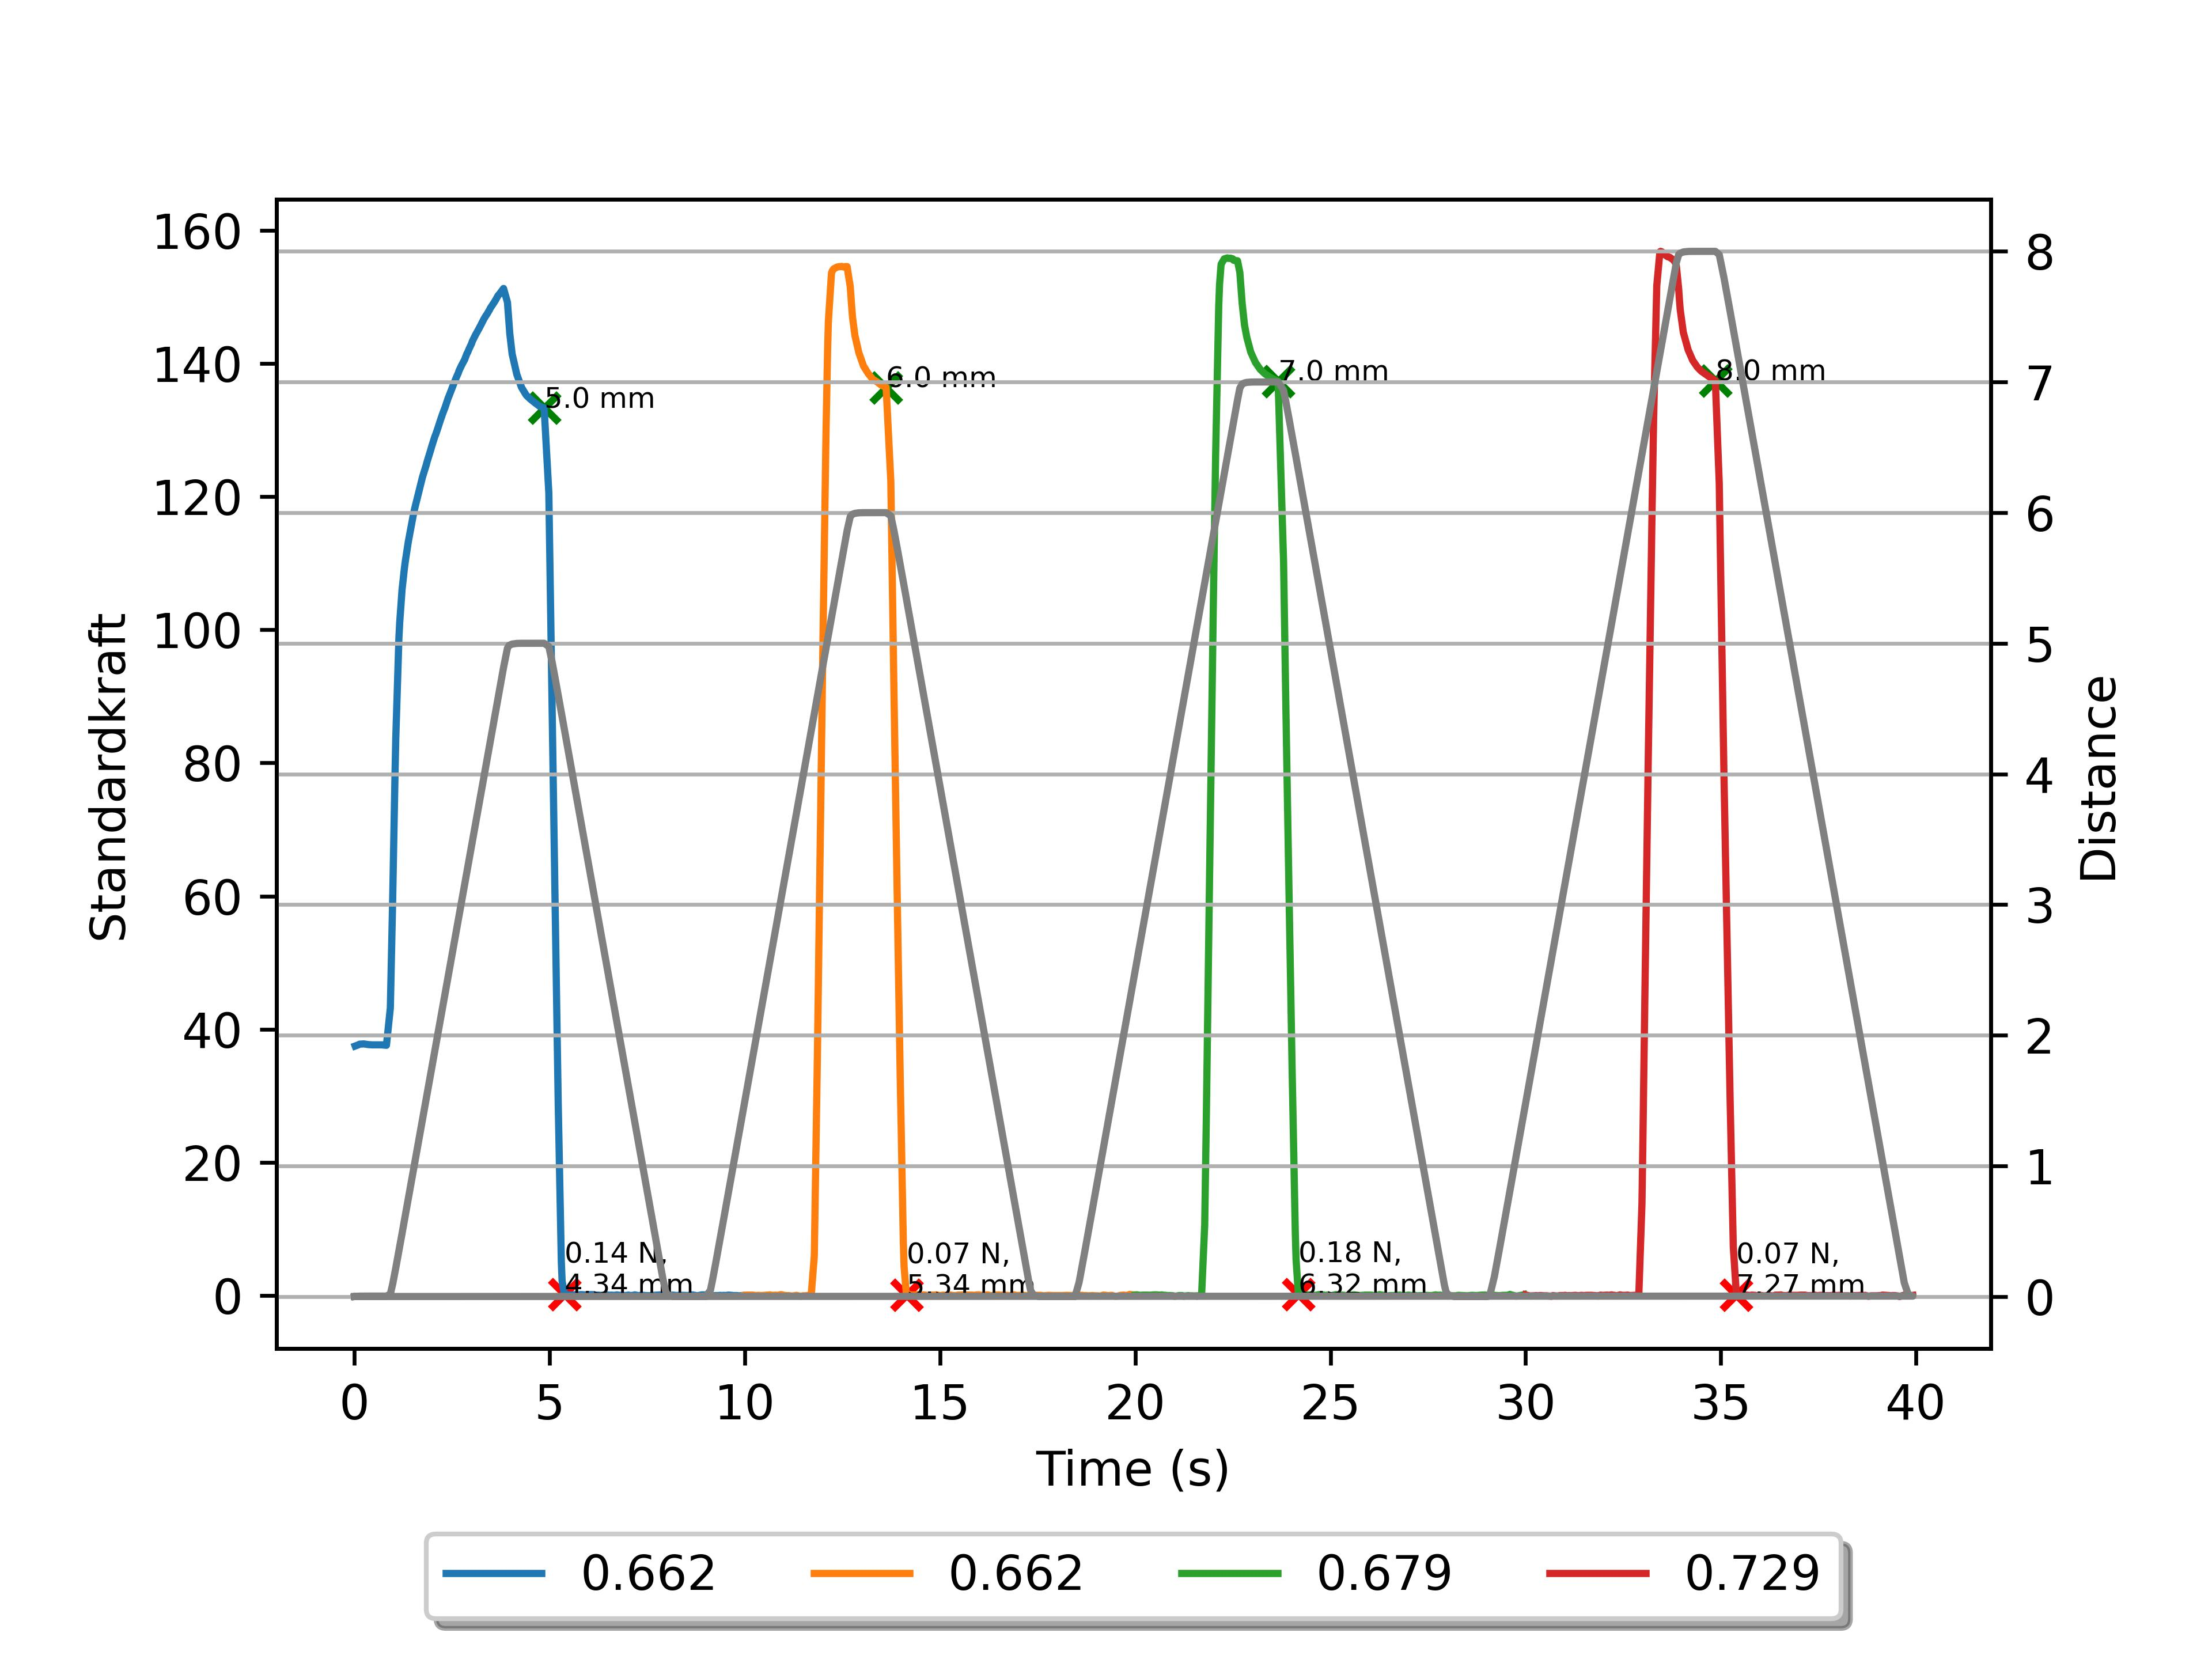
\includegraphics[width=0.9\textwidth]{springback_multiple.jpg} % first figure itself
%        \caption{Experiment: Bending one metal sheet multiple times with different $y_p$ values.}
%        \label{springback_multiple}
%    \end{minipage}\hfill
%    \begin{minipage}[b]{0.5\textwidth}
%        \centering
%        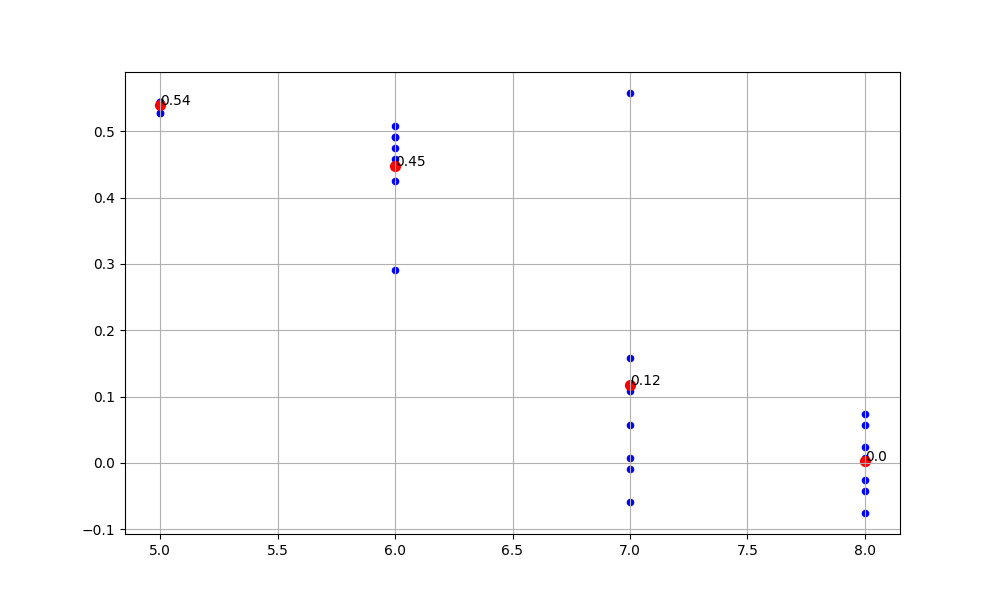
\includegraphics[width=1.1\textwidth]{springback_multiple_inconsistent_results.png} %
%        second figure itself
%        \caption{Inconsisten results bending one metal sheet mutliple times. The spread of the
%        results is very large.}
%        \label{springback_multiple_inconsistent_results}
%    \end{minipage}
%    \label{fig:springback_multiple_overview}
%\end{figure}

%\subsubsection{Bending Machine}
%Before using the three point bending machine, a brake bending machine was used to test the
%influence of the bending
%on the spring back. The brake bending machine is a machine used to bend metal sheets. It is a
%very common machine in
%the industry and is used to bend metal sheets to a specific radius. The brake bending machine
%used is a
%\textit{Bendmaster 1000} from \textit{Bendmaster}.
%
%After a series of bends it was observed, that the spring back values where much higher than
%expected. The explanation
%for that behavior was, that altering the position the bending beam of that specific machine was
%not enough to get the
%desired angle. Thus, the machine excluded for the generation of the data and the three point
%bending machine was used
%instead.
%
%Despite the inaccurate data, it was later observed, that the distribution of the spring backs was
%very similar to the
%later experiments with the three point bending machine.

\subsection{Experimental setup}\label{subsec:experimental-setup}
The experimental setup comprises of a three-point bending machine, consisting of a punch and
die, with the latter lacking a bottom, which allows only air bending metal-sheet.
The material testing machine utilized is the \textit{Zwick MX 25A}, which is equipped with a load
cell and a displacement sensor.
The load cell measures the force applied to the sheet (in $N$), while the displacement sensor
measures the displacement of the punch ($y_p$).
The punch is mounted on the top of the machine and is stationary, while the die is mounted on the
bottom and is the part which can be moved.
The machine is operated via a computer and the \textit{ZwickRöll TestXpert} software, which is
used for both machine control and data collection.

The experimental setup and the process parameters are shown in
Figure~\ref{fig:process_parameters} where $V$ is the die opening which is the opening between the
the two points between the sheet metal is placed.
The parameters $y_p$ is the punch penetration, which is the distance the punch is moved into the
sheet.
The parameter $t$ is the thickness of the metal sheet while $\alpha$ is the corresponding
angle after the bending process..
Parameter $r_p$ is the punch radius which is the radius of the tip of the punch, which was never
replaced in all experiments and therefore remains constant.


\begin{figure}[h]
    \begin{tcolorbox}[arc=0pt,boxrule=0.5pt]
        \centering
        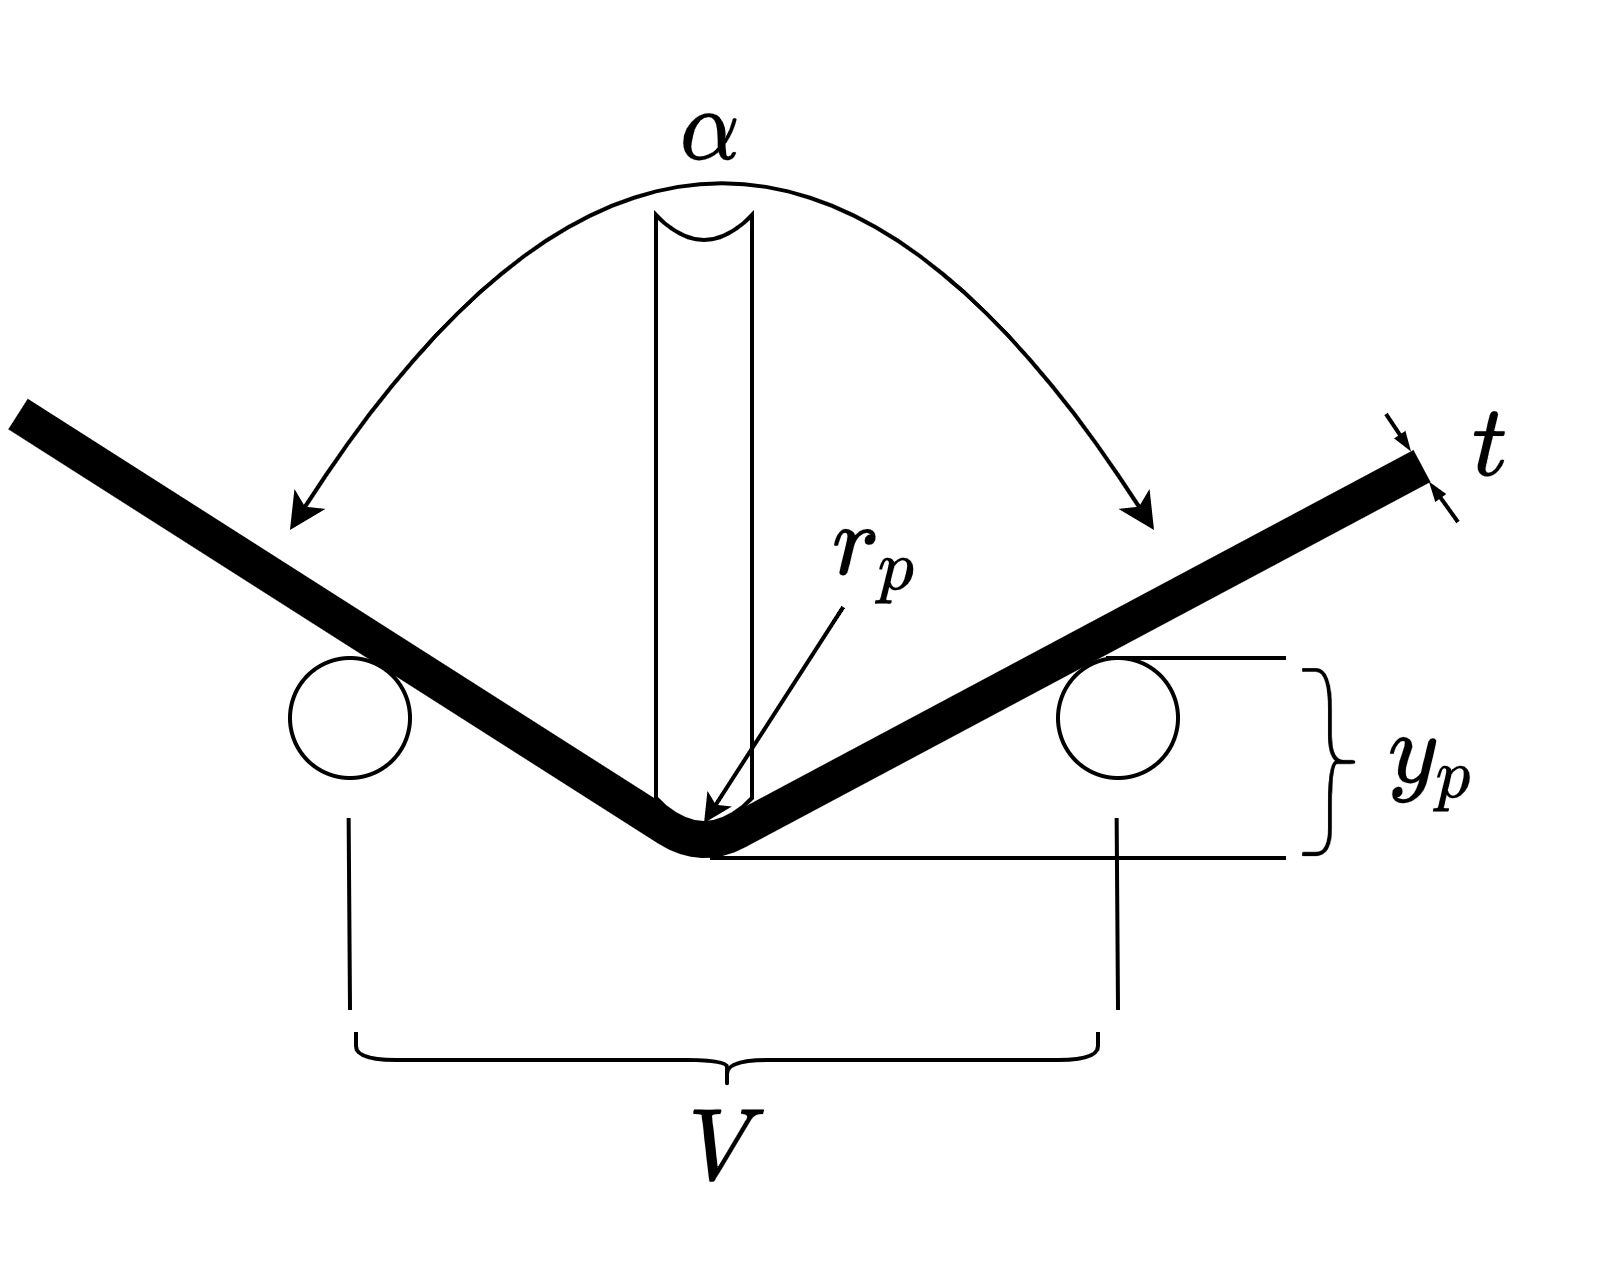
\includegraphics[trim=left botm right top, width=0.6\textwidth, clip]{process_parameters}
        \caption{Process parameters: Sheet bending angle ($\alpha$), sheet thickness ($t$), punch
        penetration ($y_p$), die opening ($V$) and punch radius ($r_p$)}
        \label{fig:process_parameters}
    \end{tcolorbox}
\end{figure}

In order to get consistent results, a number of constant and variable parameters were chosen.
The parameters include the punch-and-die tooling made of steel where die punch had a radius
($r_p$) of 5 mm and and
die radius ($r_m$) of 10 mm. The die opening $V$ was varied between 10 and 50 mm and the punch
penetration $y_p$ was
varied between 0 and 20 mm.

The machine was configured to move the punch with a constant speed of 100 mm/min until it
measured a resistance of 1 N.
That meant, that the punch reached the metal plate and the actual bending process can start.
After a hold time of 1 second the punch was moved with a slower speed of 8 mm/min until the
specified punch penetration was reached.
The length and width of the metal sheet was 100 mm and 20 mm respectively.

Using the \textit{ZwickRöll TestXpert} software, the following parameter where set for the
experiment, which are summarized in Table~\ref{tab:experimental-setup-constant-parameters}.
The punch of the machine was never replaced and therefore the radius of the punch remained
5 mm.
The width and length of metal sheets where 100 mm and 20 mm respectively.
The punch speed was set too 80 mm/min and the hold time was set to 1 second, latter is the time
the punch stays at the end of the metal sheet and has to be a least 1 second which is a limitation
of the machine.
After the bending process, the punch was moved back to the starting position with a speed of
8 mm/min.
This speed was chosen significantly lower than the speed used for the bending process
in order to accuratly measure the spring back to avoid any damage to the metal sheet.
The punch force threshold was set to 1 N, which means, that the punch starts bending the metal a
soon as it touches the sheet metal.

\begin{table}[htb]
    \begin{tcolorbox}[arc=0pt,boxrule=0.5pt]
        \sisetup{group-minimum-digits = 4}
        \centering
        \label{tab:experimental-setup-constant-parameters}
        \begin{tabular}{lll}
            \toprule
            \thead{\textbf{Parameter}} & \thead{\textbf{Values}} & \thead{\textbf{Unit}}
            \\
            \midrule
            Punch radius & 5 & $mm$
            \\
            \hdashline
            Sheet width & 20 & $mm$
            \\
            \hdashline
            Sheet length & 100 & $mm$
            \\
            \hdashline
            Punch speed & 80 &
            $mm/min$ \\
            \hdashline
            Punch speed up (after bend) & 8 &
            $mm/min$ \\
            \hdashline
            Hold time & 1 & $s$ \\
            \hdashline
            Punch force threshold & 1 & $N$
            \\
            \bottomrule
        \end{tabular}
        \caption{Constant parameters in th eperimental setup}
    \end{tcolorbox}
\end{table}

The following parameters where varied in the experiments, which are summarized in
Table~\ref{tab:experimental-setup-variable-parameters}.
The die opening $V$ was varied between 10 and 50 mm and the punch penetration $y_p$ was varied
between 0 and 20 mm.
The thickness of the metal sheet $t$ was varied between 0.5 and 2 mm.
Also the punch penetration $y_p$ was varied between 0 and 20 mm.

\begin{table}[htb]
    \begin{tcolorbox}[arc=0pt,boxrule=0.5pt]
        \sisetup{group-minimum-digits = 4}
        \centering
        \label{tab:experimental-setup-variable-parameters}
        \begin{tabular}{lll}
            \toprule
            \thead{\textbf{Parameter}} & \thead{\textbf{Values}} & \thead{\textbf{Unit}}
            \\
            \midrule
            %  \unit{(Kcal\per\mole)\squared}}} & \thead{RMSD l.b.} & \thead{RMSD u.b.}  \\
            \midrule
            Punch penetration  $y_p$ & 2.5, 5, 7.5, 10, 12.5, 15, 17.5, 20 &
            mm \\
            \hdashline
            Die opening        $V$ & 10, 20, 30, 40, 50
            & mm \\
            \hdashline
            Thickness          $t$ & 0,5, 1, 1.5, 2, 2.5, 3
            & mm \\
            \bottomrule
        \end{tabular}
        \caption{Varying parameters in the experimental setup}
    \end{tcolorbox}
\end{table}

\subsection{Measuring The Spring Back} \label{subsec:measuring_the_spring_back}
The output data contained different data points, which were used to calculate the spring back.
Important parameters for the calculation are the force, punch penetration and testing time.
As shown in Figure~\ref{fig:springback_measured} at the $y_p$ maximum the punch penetration and
the force are
maximized as well. The punch stays at that position for 1 second and then moves back with a
slower speed. This hold
time a limitation of the machine and can not be changed.
After the punch is moved back, the force is reduced and the punch penetration is reduced as well,
until the punch is
at the initial position. For a short time after the lift, the load cell still measures a force.
That is because the
metal sheet springs back and the punch is still in contact with the sheet. This was measured
using a python script,
the green and the yellow point represent the resulting spring back distance.

\begin{figure}[H]
    \begin{tcolorbox}[arc=0pt,boxrule=0.5pt]
        \centering
        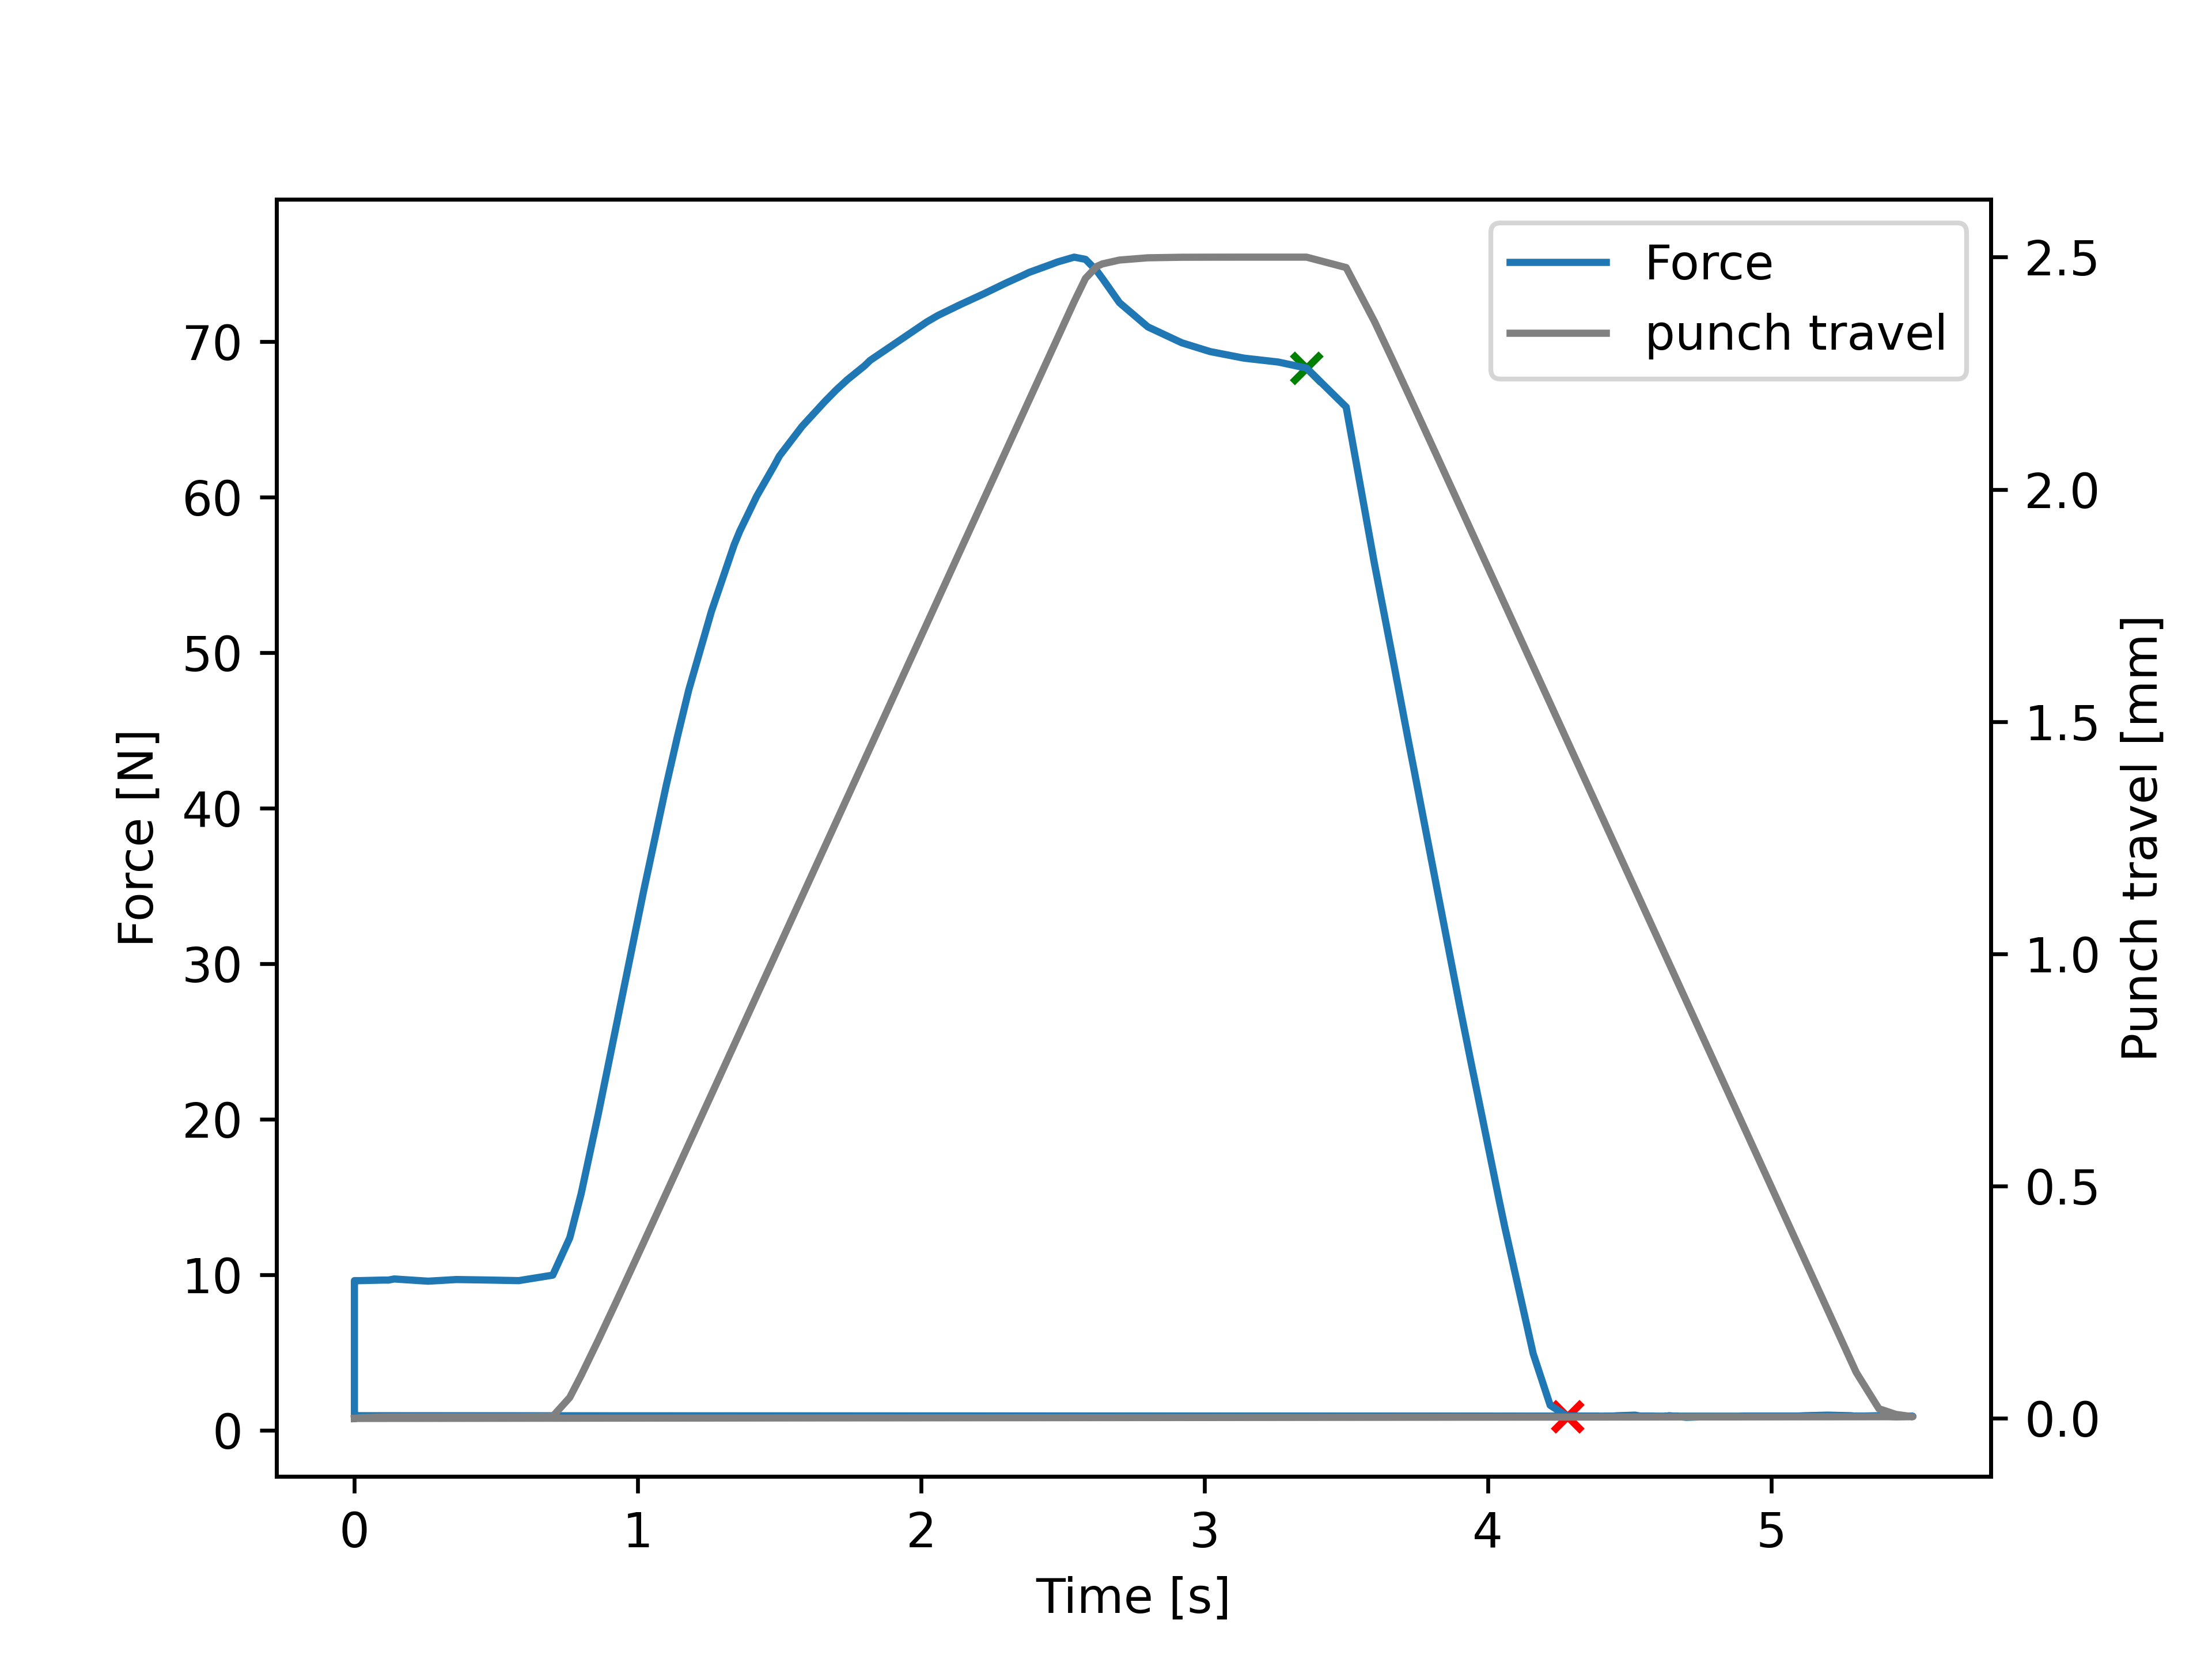
\includegraphics[width=0.9\textwidth]{springback_measured}
        \caption{A steel metal sheet was bent with a punch penetration of 5 mm the spring back is 0
        .37 mm. The blue line
        shows the force and the blue line shows the punch penetration.}
        \label{fig:springback_measured}
    \end{tcolorbox}
\end{figure}

\subsubsection*{\textit{Notes}}
\begin{itemize}
    \item \textit{Why is an initial force measured before the punch is moved?}
    \item \textit{TODO: Add legend for grey line (punch penetration) and blue line (force))}
    \item \textit{TODO: More dpi for the image}
\end{itemize}


\begin{filecontents*}{example.dat}
    Method Pink-1C Pink-AC Green-1C Green-AC Blue-1C Blue-AC Cyan-1C Cyan-AC Red-1C Red-AC
    Orange-1C Orange-AC
    Square 24.75 4.8 32.28 7.39 32.65 7.53 31.96 7.18 33.57 8 33.19 7.08
\end{filecontents*}


\label{sec:dataset_exploration}

\subsection{Adding Features to the Dataset}\label{subsec:adding-features-to-the-dataset}
The current dataset includes three independent and one dependent feature. These features
will be discussed in more detail in the following section.
On goal was it to enhance the dataset with more features, this would improve
the performance of models and provide greater insight into the bending process.

On potential candidate for a new feature is the tension. A drawing test was carried out for this
which is described more in detail in the next section...

\subsubsection*{\textit{Notes}}
\begin{itemize}
    \item \textit{TODO: Add drawing test}
\end{itemize}

\subsection{Dataset Exploration}\label{subsec:dataset-exploration}

\subsubsection{Features}
The output data of the bending machine contained 26 features which can be found in the appendix.
Out of these
features only the standard power and the distance $y_p$ and the force are relevant for
calculating the spring back
which was described in the last section \ref{subsec:measuring_the_spring_back}.
The final dataset therefore contained 3 features plus the added spring back.
In total 396 data points where crated using the described approach.
An example of the dataset is shown in Table~\ref{tab:dataset_example}.

\begin{table}[h]
    \begin{tcolorbox}[arc=0pt,boxrule=0.5pt]
        \sisetup{group-minimum-digits = 4}
        \centering
        \label{tab:dataset_example}
        \begin{tabular}{l|llll}
            \toprule
            \thead{\textbf{index}} & \thead{\textbf{Distance}} & \thead{\textbf{Spring Back}} &
            \thead{\textbf{Thickness}}
            & \thead{\textbf{Die Opening}}
            \\
            1   & 5   & 0.6667 & 2.0 & 50  \\
            \hdashline
            2   & 15  & 0.9164 & 2.0 & 50  \\
            \hdashline
            3   & 10  & 0.6829 & 2.0 & 50  \\
            \hdashline
            ... & ... & ...    & ... & ... \\
            \hdashline
            396 & 5   & 0.6667 & 3.0 & 10  \\
            \bottomrule
        \end{tabular}
        \caption{Varying parameters in the experimental setup}
    \end{tcolorbox}
\end{table}

With 100 estimators in \ac{RF} a \ac{MSE} of 0.15 and \ac{RMSE} 0.39 was achieved.
Figure~\ref{fig:rf_feature_importance} compares and visualizes the relative importance of the
features used for
training the model.
As shown, the thickness is the most important feature followed by distance and die open. The
results show, that all
three featured are relevant for the outcome and so no feature can be removed from the dataset to
get a better
performance of the model.

\begin{figure}[htb]
    \begin{tcolorbox}[arc=0pt,boxrule=0.5pt]
        \centering
        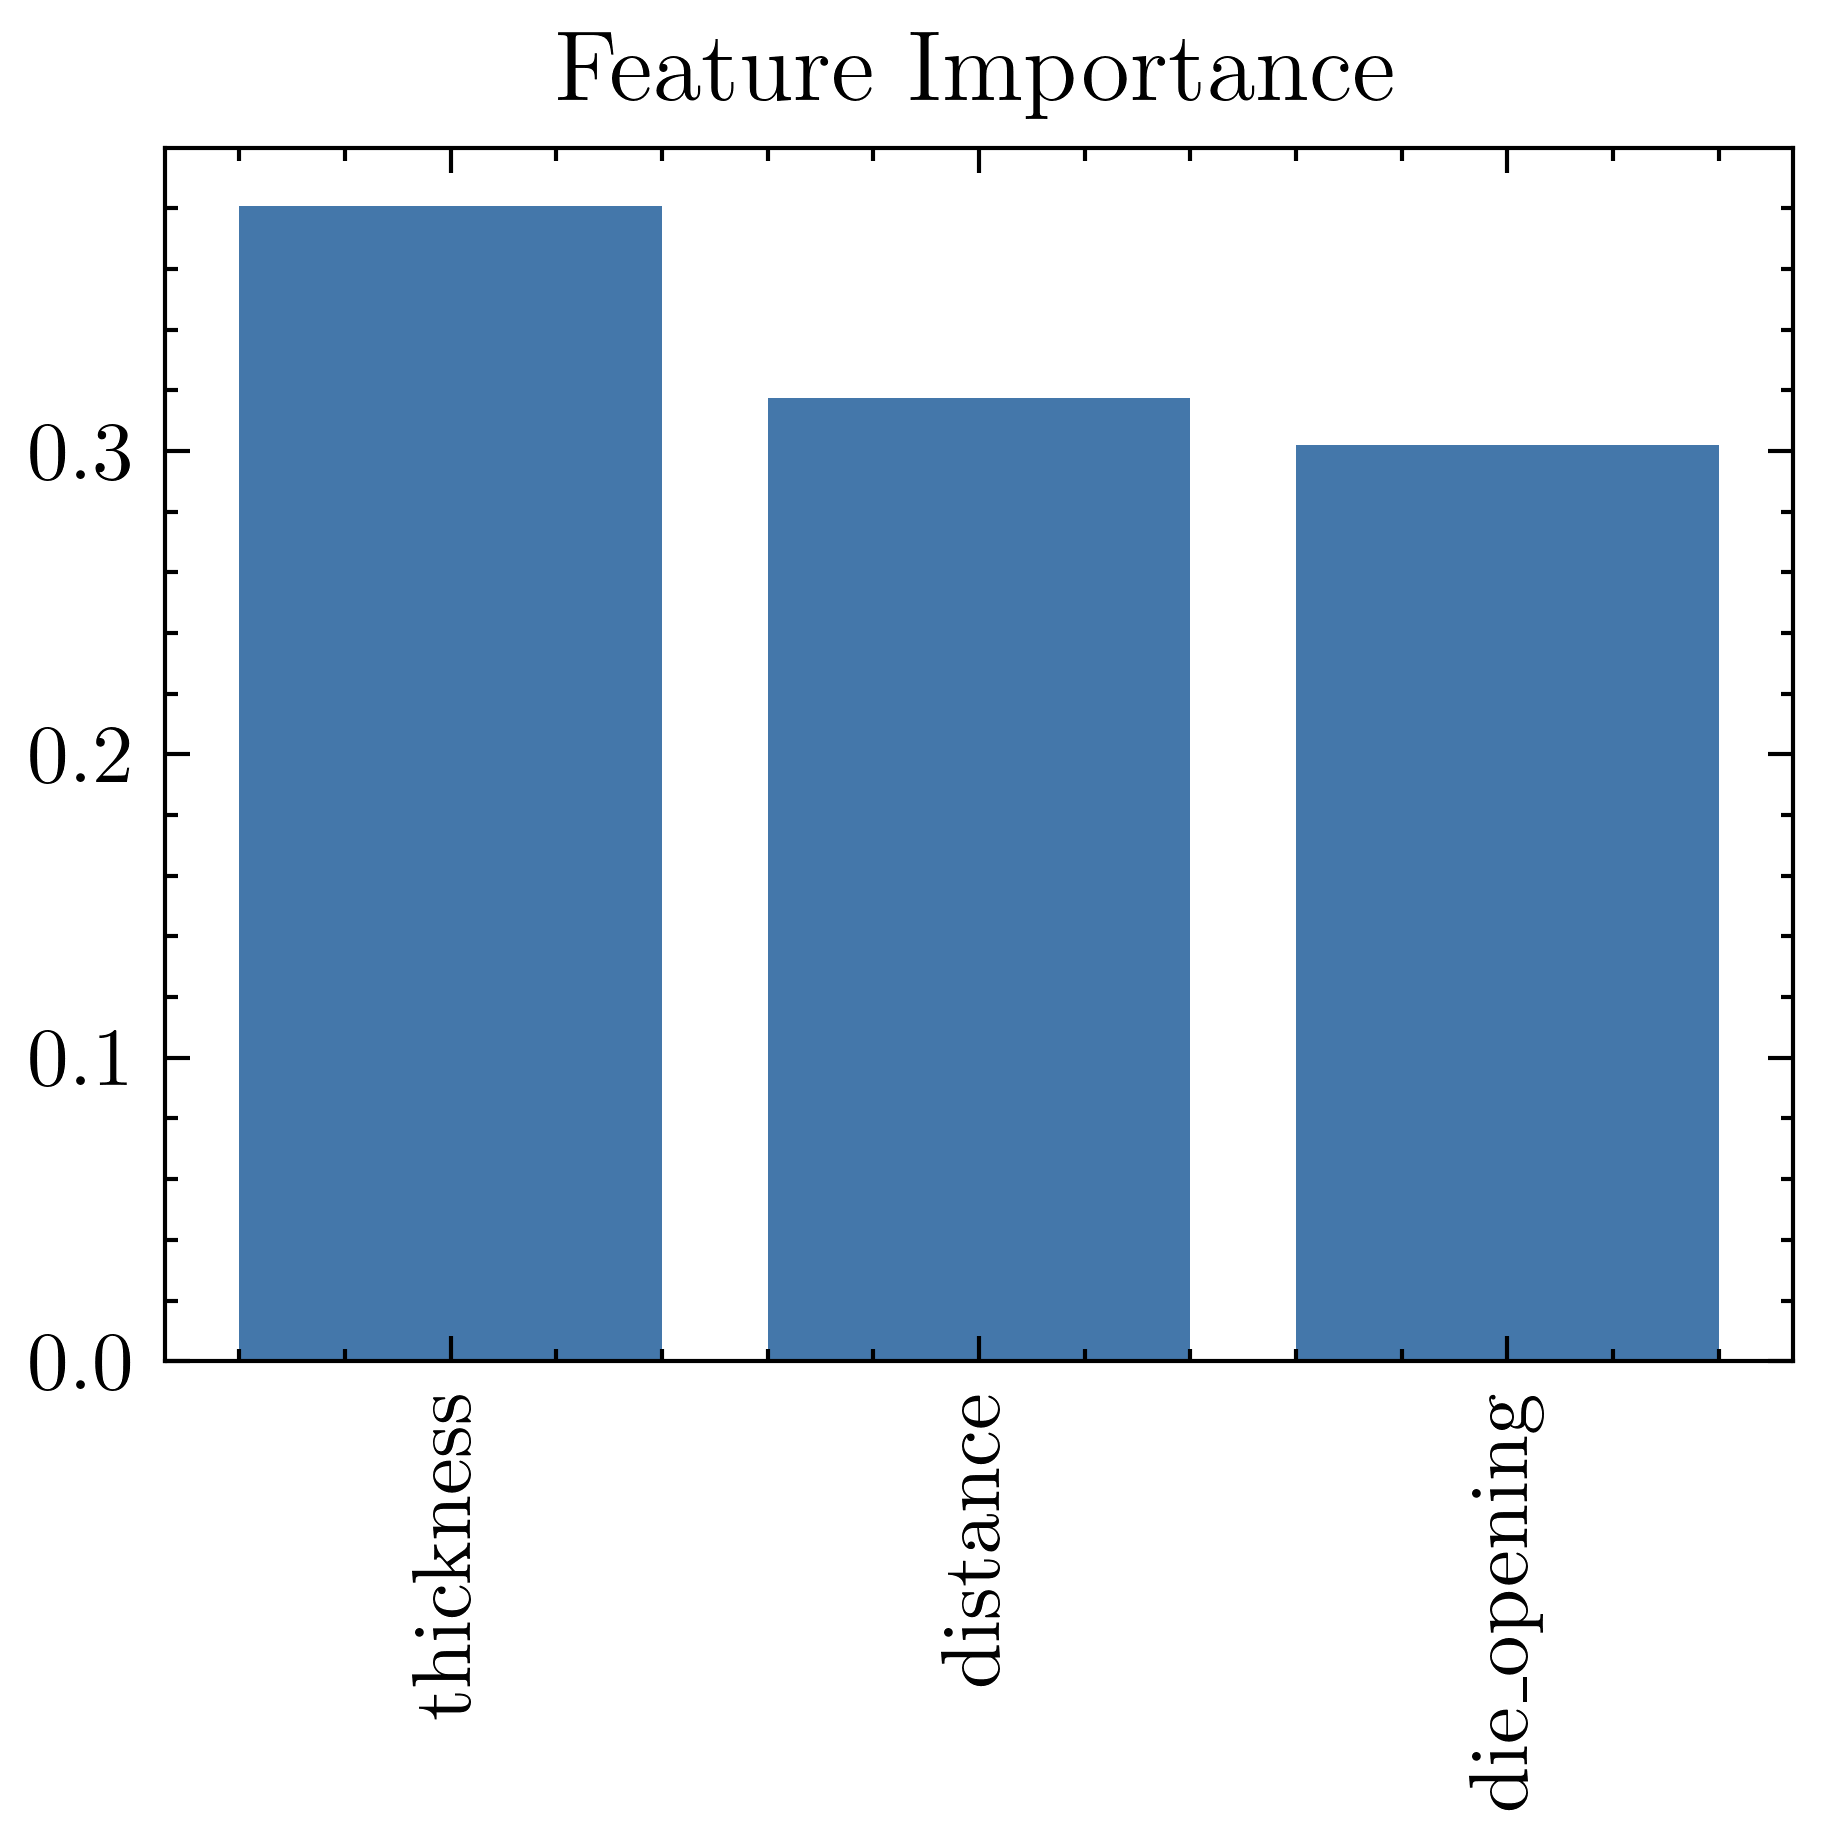
\includegraphics[width=0.6\textwidth]{Random_Forest_Regression_importances}
        \caption{Relative feature importance}
        \label{fig:rf_feature_importance}
    \end{tcolorbox}
\end{figure}

\subsection{Visualizing The Data}\label{subsec:visualizing-the-data}
Figure~\ref{fig:v30_springbacks} shows the spring backs for the $V30$ dataset.
In general, it can be seen that the spring backs is less for lower thicknesses and higher for
higher thicknesses.
Also, the spring backs for lower thickness tend to go up with increasing punch penetration, while
the spring backs
for higher thicknesses tend to go down with increasing punch penetration.

The factors for the behavior of the spring back can't be fully understood with the available
data, which makes it a
good case for machine learning.

\begin{figure}[htb]
    \begin{tcolorbox}[arc=0pt,boxrule=0.5pt]
        \centering
        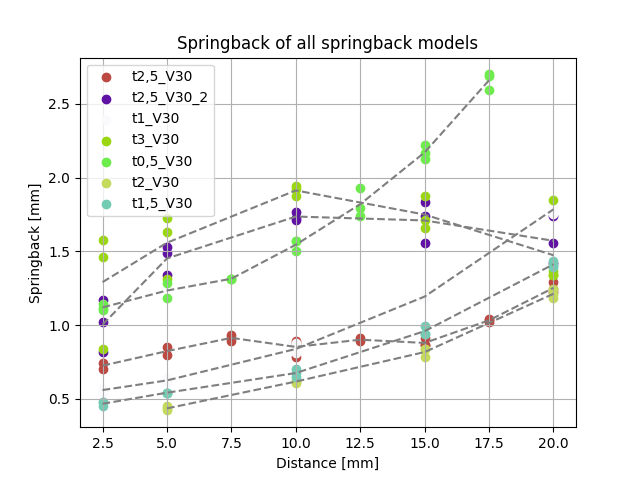
\includegraphics[width=0.8\textwidth]{V30_all_springbacks}
        \caption{Springbacks for $V30$}
        \label{fig:v30_springbacks}
    \end{tcolorbox}
\end{figure}

\subsubsection*{\textit{Notes}}
\begin{itemize}
    \item \textit{TODO: Add better picture. Ordered by $t$, better colors, scienceplot, punch
    penetration instead of spring back}
    \item \textit{Experimental setup methodology like Jonas.}
\end{itemize}

\subsubsection{Data Quality}
The dataset was created in an experimental environment and the samples where carefully measured.
Therefor the dataset does not contain many outliers and the data quality is high.

As shown Figure~\ref{fig:train_test_split} data for all possible $V$ and $t$ combinations where
collected. Also there
the $y_p$ values are evenly distributed and always range from 2.5 to 20 mm.
Furthermore, the dataset was continuously extended with new data points throughout the project.
During this process
multiple outliers and wrong measurements where detected and removed.

It has to be noted that therefore the dataset does not model a real-world scenario, where the
data quality is not as
high as in the experimental environment.
This has been considers in section~\ref{sec:robustness}~Robustness, where artificial noise is
added to the dataset to
test the robustness of the models.

\subsubsection*{\textit{Notes}}

\begin{itemize}
    \item \textit{The Figure feature importance was created using a random forest so it does not
    belong here. Find a
    \item different method to visualize the feature importance.}
    \item \textit{Add example picture of spring back plots}
    \item \textit{It is not yet decided if artificial noise will be added to the dataset.}
    \item \textit{Add some data quality measure?}
\end{itemize}

\subsection{Data Preprocessing}\label{subsec:data-preprocessing}

The three independent features $y_p$, $V$ and $t$ as well as the dependend feature $spring\_back$
were normalized
using the \texttt{MinMaxScaler}from the scikit-learn library. The \texttt{MinMaxScaler} scales
the data between 0 and
1. The scaler was fitted on the training data and then used to transform the test data. The
scaler was saved to be
used for the prediction of the spring back of the real world data.

Scaling is only done on the training data, because cross-validation is later used to tune and
evaluate the models.
Scaling the whole data set before the split would lead to data leakage because the min and max
values of the test
data would be used to scale the training data.
How the data was split can be seen in Figure~\ref{fig:train_test_split}.

Because cross-validation is later used to tune and evaluate the models the data was split before
the scaling. How the
data was split can be seen in Figure~\ref{fig:train_test_split}.

\subsubsection*{\textit{Notes}}
\begin{itemize}
    \item \textit{TODO: Outlier handling is not done and mentioned. Is this necessary?}
    \item \textit{TODO: Use more sophisticated scaling methods, not only min-max scaling. For
    example for V
    classfication}
\end{itemize}


% Pado: This is a little confusing - does the Y axis show the force? Why is the blue line the
% shape it is? Is it
% maybe two separate lines, the movement of the punch and the reaction of the metal?

\subsection{Computational Setup}
For training the machine learning models a ThinkPad X1 Carbon 2019 with an Intel Core i7-10610U
CPU @ 1.80GHz and 16
GB RAM was used. The operating system used is Ubuntu 20.04.2 LTS. The code for the model is
written in Python 3.8.5
using the IDE PyCharm. The libraries used are mentioned in Table~\ref{table:libraries}.

\captionsetup{width=1\textwidth}

\begin{table}[htb]
    \begin{tcolorbox}[arc=0pt,boxrule=0.5pt]
        \sisetup{group-minimum-digits = 4}
        \centering
        \label{table:libraries}
        \begin{tabular}{ll}
            \toprule
            \thead{\textbf{Library}} & \thead{\textbf{Version}} &
            \toprule
            numpy & 1.23.2 \\
            \hdashline
            pandas & 1.5.1 \\
            \hdashline
            matplotlib & 3.6.2 \\ \hline
            \bottomrule
        \end{tabular}
        \caption{Libraries used for the machine learning models.}
    \end{tcolorbox}
\end{table}

Looking at the correlation matrix shown in Figure~\ref*{fig:correlation_matrix} it can be seen,
that the distance and
the spring back are more correlated than the other features. This is expected, because the punch
penetration $y_p$ is
the main factor which influences the spring back. The other features are not correlated with each
other, no
multicollinearity is present which is good for the machine learning models.

\begin{figure}[H]
    \begin{tcolorbox}[arc=0pt,boxrule=0.5pt]
        \centering
        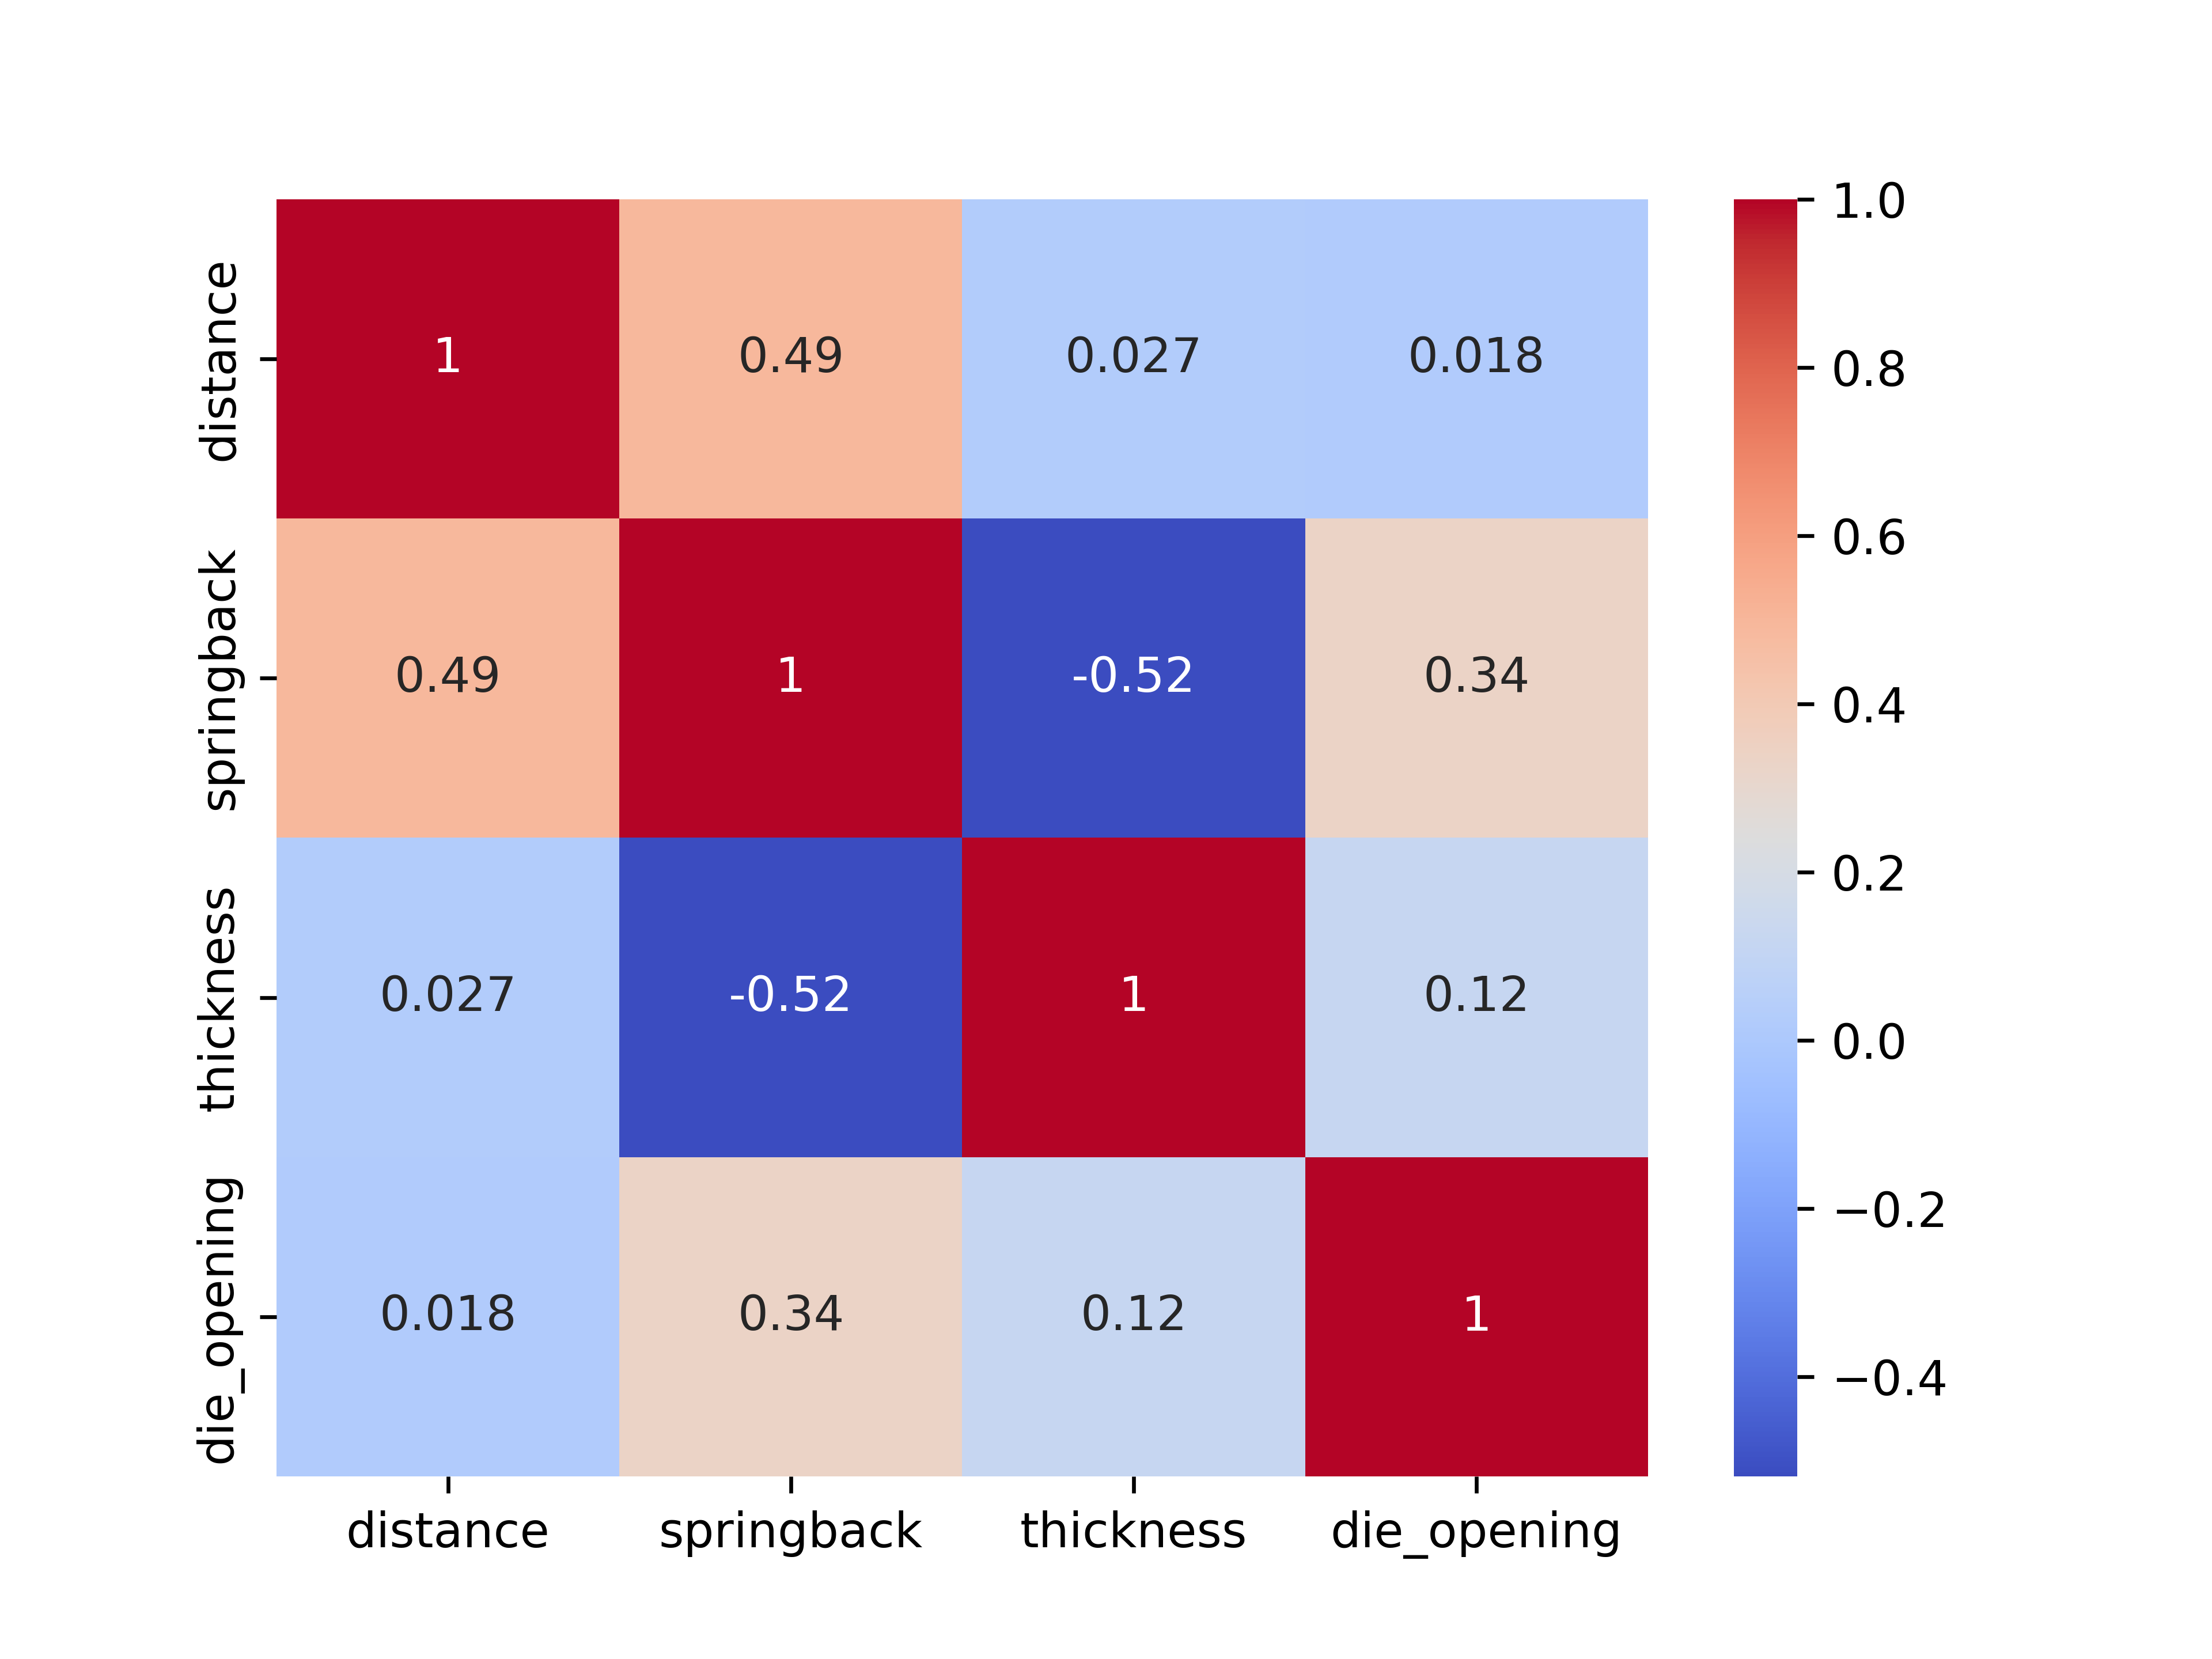
\includegraphics[width=0.8\textwidth]{correlation_matrix}
        \caption{Correlation matrix}
        \label{fig:correlation_matrix}
    \end{tcolorbox}
\end{figure}


\section{Model Selection}\label{sec:model-selection}

\subsection{Support Vector Regression (SVR)}\label{subsec:support-vector-regression-(svr)}
Support Vector Machines \ac{SVM} are usually used for classification problems. The \ac{SVM}
algorithm is used to find
a hyperplane in an N-dimensional space (N - the number of features) that distinctly classifies
the data points.
\cite[p. 42]{awad_efficientlearningmachines_2015}
Predicting the spring back is a regression problem, so the \ac{SVM} algorithm need to be
generalized of
classification problems, where the model returns continuous values instead of finite set of values.
This is done by using the \ac{SVR} algorithm, which is inspired by  \ac{SVM} and uses the same
principles.
It fits a model to data using only residuals smaller in absolute value than a certain constant
called
$\epsilon$-sensitivity

This is done by creating a "tube" of $\epsilon$ width around the data, with points inside the
tube not being
penalized and points outside the tube being penalized based on their distance from the predicted
function.
This is done similar to how \ac{SVM}s penalize points in classification.
Like \ac{SVM}, \ac{SVR} fins a well-fitting hyperplane to a kernel-induced feature space to
achieve good
generalization performance using the original features.
\cite[p. 369]{montesinoslopez_supportvectormachines_2022}

\subsubsection*{Kernel Trick}

The kernel trick is a method to transform the data into a higher dimensional space, where the
data is linearly
separable.
This is done by using a kernel function, which is a function that maps the data into a higher
dimensional space.
Two methods are usually used for \ac{SVM}s, the polynomial kernel and the radial basis function,
also known as gaussian kernel.
\cite[p. 97-98]{muller_introductionmachinelearning_2016}
In practise the mathematical details behind these kernels are not important, but it is important
to know that they are used to transform the data into a higher dimensional space, where the data
is linearly separable.

\subsection{Multi Linear Regression}\label{subsec:multi-linear-regression}

\subsection{Polynomial Regression}\label{subsec:polynomial-regression}

\subsection{Decision Tree Regression}\label{subsec:decision-tree-regression}

\subsection{Random Forest Regression}\label{subsec:random-forest-regression}
% Erst einmal auf decision tree generell eingehen
A commonly used method in machine learning. The goal is to solve classification or regression
problems by predicting
the value of a output variable by one or multiple input variables. \cite[p.
253]{shaik_briefsurveyrandom_2019}
To build a \ac{DT} the source dataset represents the root node of the tree this data set is split
into leafs
(children) by using a set of spitting rules until each leaf in the \ac{DT} is "pure" and only
contains one target
value. Depending on the use cases this is a single class or a single regression value. \cite[p.
70-72]{muller_introductionmachinelearning_2016}
% -> Problem von decision tree 
The main drawbback of \ac{DT}s is the tendency to overfit and poor generalization performance,
what makes them not
paticaly for most use cases. Therefore usualy ensemble methods are used instead of a single
\ac{DT}. \cite[p.
78]{muller_introductionmachinelearning_2016} \cite[p. 251]{liu_newmachinelearning_2012}
% -> Warum random forst das problem löst 
Random forest \cite[]{breiman_randomforests_2001} is a type of ensemble learning algorithm in
which multiple decision
trees, which are "weak learners," are trained and combined to produce a more accurate and stable
prediction, known as
a "strong learner." \cite[p. 24]{awad_efficientlearningmachines_2015}
The risk of overfitting is mitigated by subset and feature randomization. Each root node uses a
unique subset of the
data and each leaf is split using a random features. This ensures that no single tree sees all of
the data, allowing
the model to focus on general patterns rather than being sensitive to noise. \cite[p.
251]{liu_newmachinelearning_2012}
% -> Beschreibung Random forest / Random foret regression 
In this supervised learning method,
%which was influenced by the research of Amit and Geman (1997), Ho (1998), and Dietterich (2000), 
a "divide and conquer" approach is used. This involves dividing the data into smaller samples,
incrementally building
a randomized tree predictor for each sample, and then combining (aggregating) these predictors
together. This
approach has proven to be effective. Because not only one but multiple classifiers are used the
random forest
learning is known as ensemble model. \cite[p. 254]{shaik_briefsurveyrandom_2019}

% -> Vorteile / Nachteile Random Forest 
This mechanism is flexible enough to handle classifications and regression problems, this is one
of the reasons that
random forests count to the most successful \ac{ML} methods. \cite[p.
3-4]{biau_randomforestguided_2016} \cite[p.
25]{breiman_randomforests_2001}

%
% Advantages
%
Random forests are a type of machine learning algorithm that uses bagging and the random
selection of features to
produce accurate results. They are effective at handling noise and can work with both continuous
and categorical
variables. This combination of techniques helps improve the performance of the algorithm. \cite[p.
259]{liu_newmachinelearning_2012}
Decision trees have a limitation in their ability to overfit, which is a disadvantage. This is
mitigated by the use
of subset and feature randomization. Specifically, each base model uses a unique subset of the
data, and each node in
the decision tree is split using a random set of features. This ensures that no single tree sees
all of the data,
allowing the model to focus on general patterns rather than being sensitive to noise. \cite[p.
259]{liu_newmachinelearning_2012}

% Bagging technique helps the algorithms performance. 
% Works well out of the box with no hyperparameter tuning.
% Fast, robust, and can show feature importances which can be quite useful.

% Disadvantages
%

% Boosted algos usuallaly outperform Random Forest.
% RF is not able to extrapolate based on the data. It can only predict within the range of the
% training data.
% Random forest regressor is unalbe to discover trens that would enable it in extrapolating
% values that fall outside
% of the training set.

%  Extrapolating is the process of estimating or predicting something beyond the range of
%  available data. (chatgpt)

%
% Alogithm steps 
%

% The following Random Forest Algorithm [9] gives the steps in constructing the
% decision trees.
% • Take N as the number of training data instances in the samples. Let M be the
% number of attributes in given input dataset.
% • Let m be the Number of parameter in the input that determines the next attribute
% to be chosen at each tree node; (where mislesserthan M).
% • The training samples are taken and a tree is constructed for each sample with
% replacement.
% • For tree node, arbitrarily select m attributes in that particular node.
% • The best split is computed based on the m input attributes of the sample dataset.
% • Each tree is grown without pruning.
% \cite[p. 254-255]{shaik_briefsurveyrandom_2019}

% A random forest does not require any cross verification and it is not over-fitting [8]. The
% Random forest uses Adaboost and Bootstrapping techniques to construct multiple
% classifiers. \cite[p. 254]{shaik_briefsurveyrandom_2019} 


% In a classification random forest, each tree in the forest makes a prediction for the class
% label of a given
% example, and the final prediction is made by majority vote, with the class label that receives
% the most votes being
% chosen as the prediction. In a regression random forest, each tree in the forest makes a
% prediction for the
% continuous value, and the final prediction is made by averaging the predictions of all the
% trees in the forest.
% (chatgpt)

% In both cases, the random forest model creates a large number of decision trees and trains them
% on different
% subsets of the training data. The decision trees are trained using a technique called bagging,
% which involves
% randomly selecting a subset of the training examples for each tree and training the tree on
% that subset. The idea
% behind bagging is to train each tree on a slightly different subset of the data, which can help
% to reduce
% overfitting and improve the overall performance of the model. (chat gpt)

\subsubsection{Gradient Boosting Regression Tree}
A gradient boosting regression is a type of ensemble learning algorithm in which multiple
decision trees are combines
to produce a more accurate and stable prediction. Similar to the random forest algorithm gradient
boosting combines
multiple weak learners to create a strong learner.
The difference to a random forest is, that the trees are trained in a serial manner and each tree
corrects the errors
of the previous tree. \cite[p. 88-89]{muller_introductionmachinelearning_2016}
Gradient boosted tree use strong pre-pruning and therefore produce shallow trees with a depth of
one to five. This
brings the advantage of a smaller model which uses less memory and also results in a faster
prediction.
Usually generating more trees improves the overall performance of the model. \cite[p.
88-89]{muller_introductionmachinelearning_2016}
Also the algorithm performs well without scaling the dataset and can handle a mixture of binary
and continuous
features. \cite[p. 88-89]{muller_introductionmachinelearning_2016}
Like other tree-based models it does not perform well on high-dimensional data.

\subsubsection*{Results}

\label{sec:model-training}


\section{Model Training}

\subsection{Training-Test Split}\label{subsec:training-test-split}
Figure~\ref{fig:train_test_split} shows the data set and which parts of it is used for training
and testing the used
models. Samples with a die opening of 30 are used to test the performance and the remaining part
is used for training.
A different approach would be to us a random test and train split, this would lead to a better
performance of the
models but would not evaluate their ability to predict new data of a different die opening.
The die opening 30 was chosen because it is in the middle of the selected data set and therefore
the models should be
able to predict the data of this die opening.
It is expected that this approach will lead to improved model performance as the data removed
lies in the middle of the parameter space.
This should result in the model generalizing better on that specific range of data as it has not
been over-exposed to it during the training process.

All models are trained with the same data set and the same parameters. The only difference is the
used algorithm.

\begin{figure}[H]
    \begin{tcolorbox}[arc=0pt,boxrule=0.5pt]
        \centering
        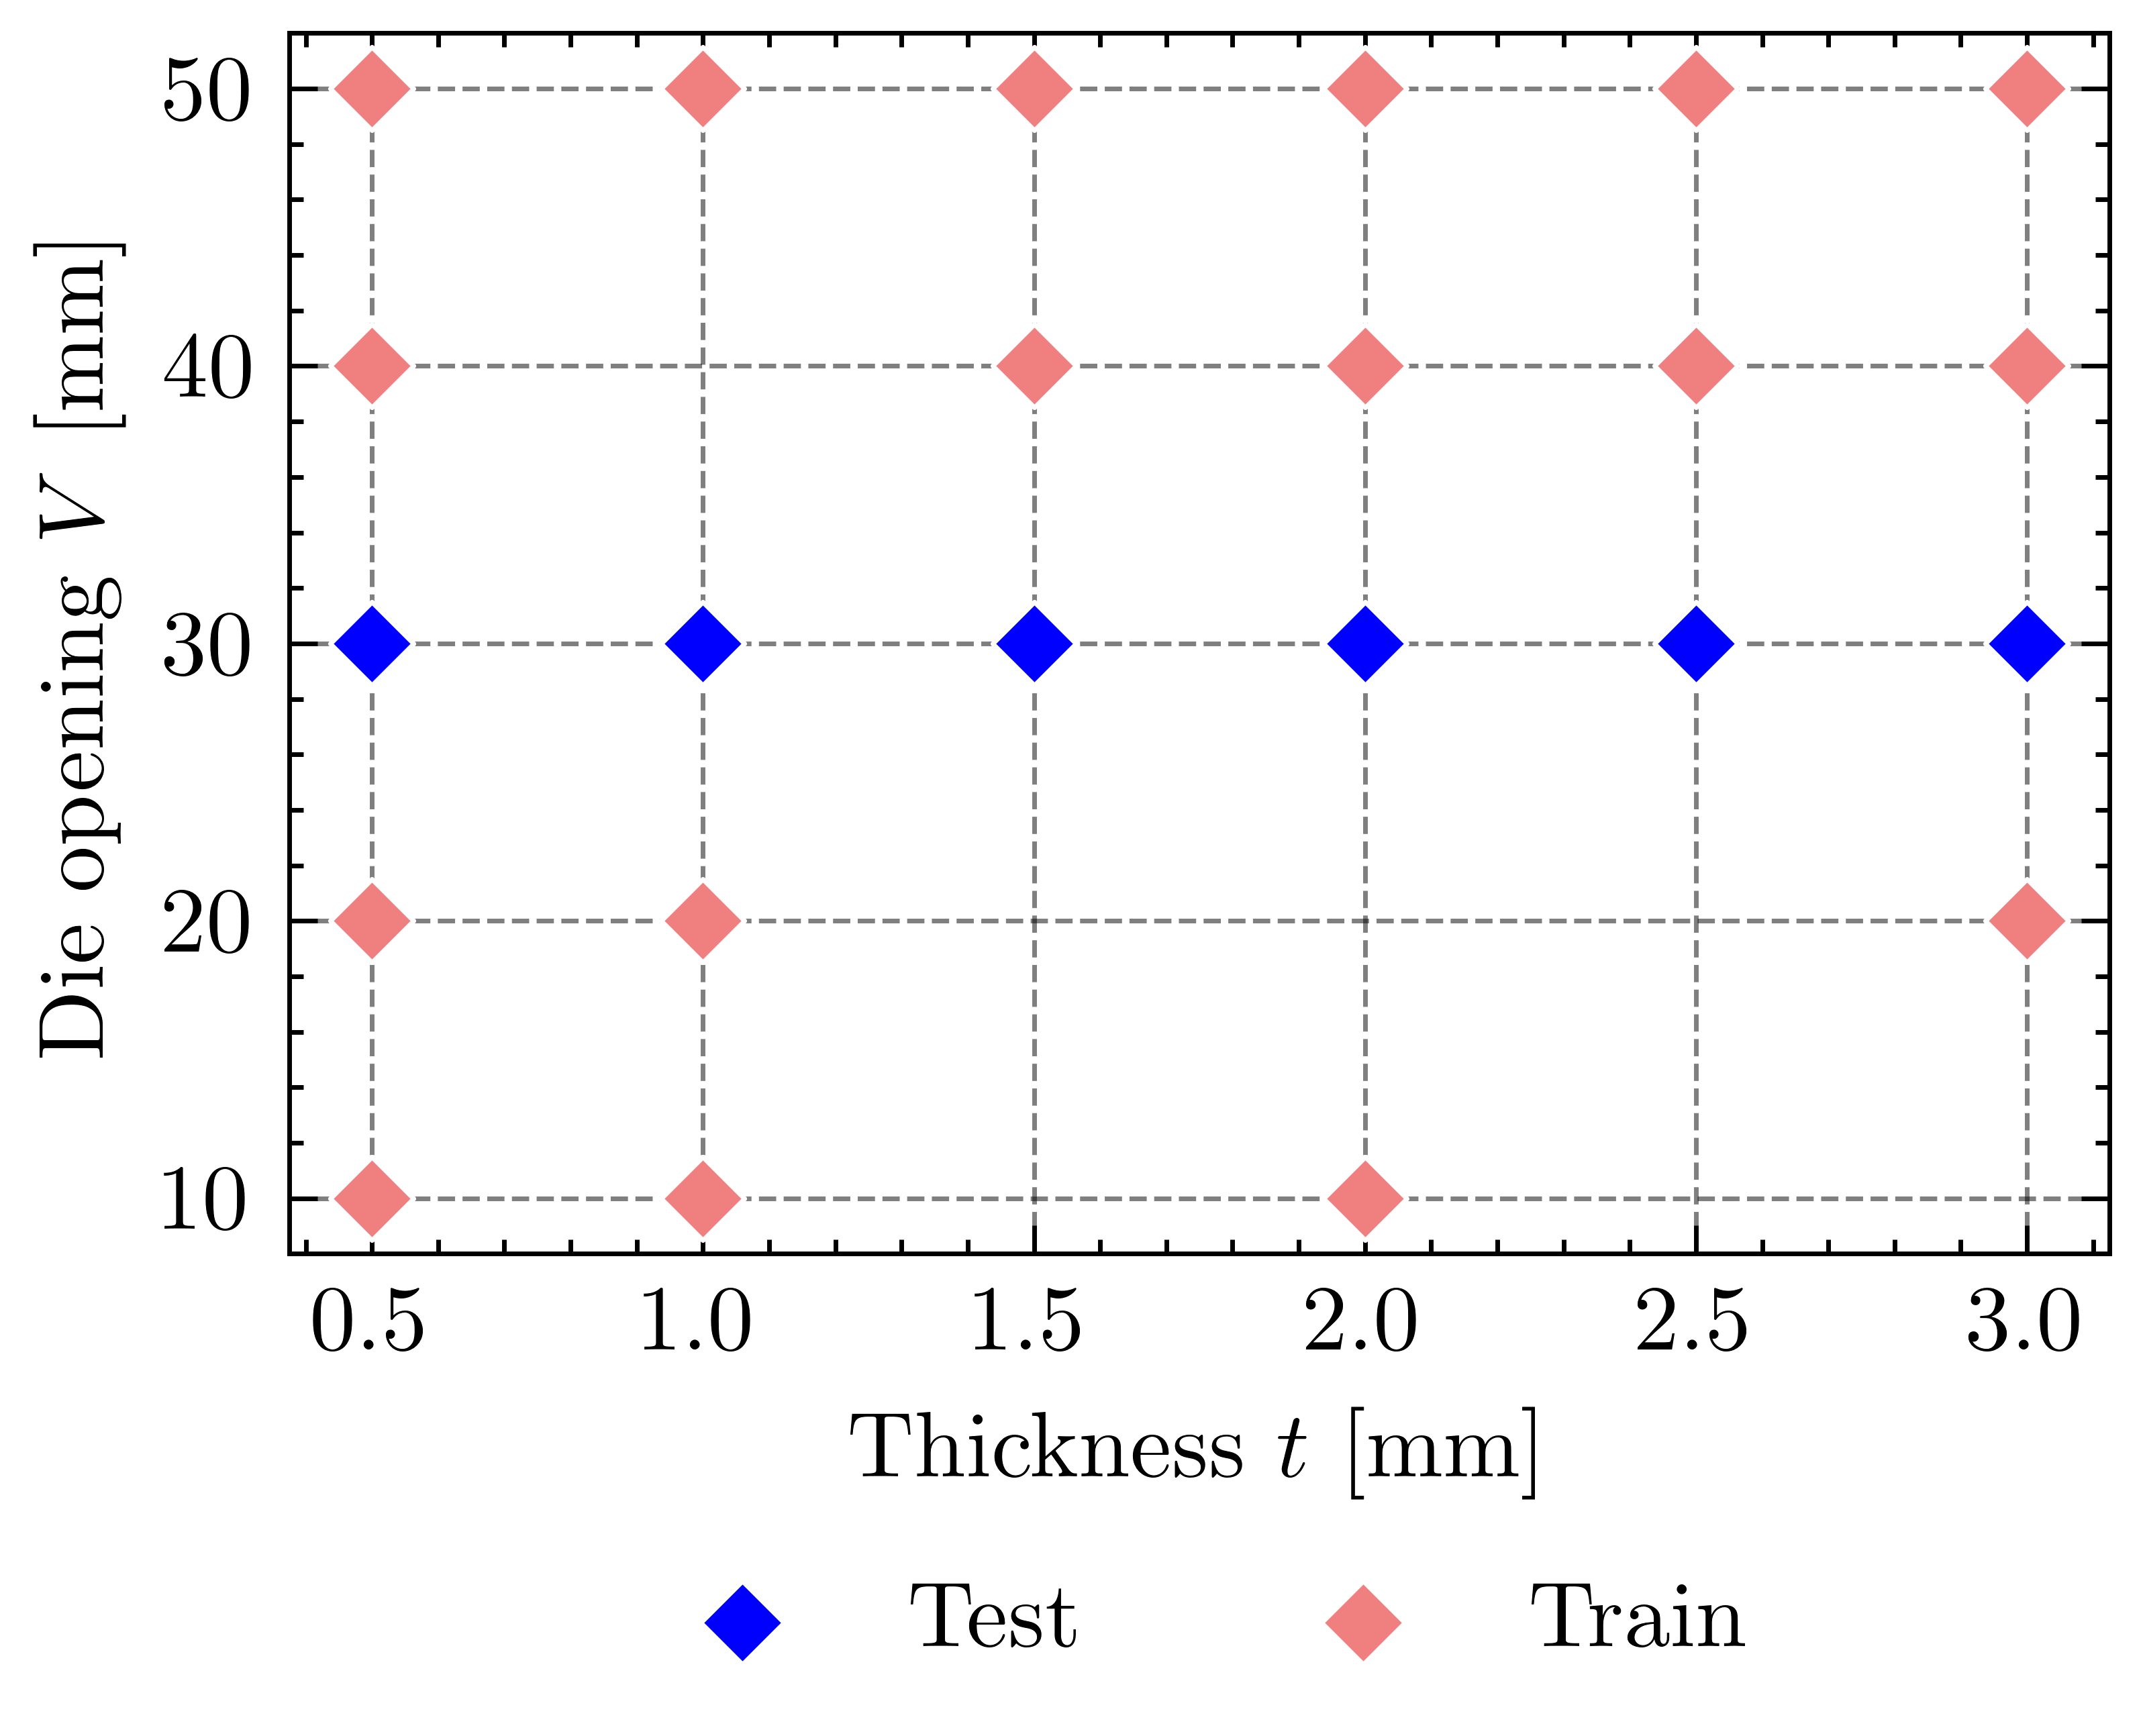
\includegraphics[width=0.8\textwidth]{test_train_split}
        \caption{The training and test dataset. (Data especially for V40 is still missing)}
        \label{fig:train_test_split}
    \end{tcolorbox}
\end{figure}

Additional to the data split shown in Figure~\ref{fig:train_test_split} a random test split was
used to train the
models. The random 80/20 split was also used to evaluate the performance of the models and to
compare them to each
other.

The reason for choosing to different methods for the data split is that the first one is used to
evaluate the models'
ability to generalize on new data. The second one is used to evaluate the models' performance on
the data set.
Also in real-world applications is possible that there is already data for all needed
$V-t$-combinations and models
could be trained on that data.

It is expected that the models perform better on the random data but the information gain about
the models' ability
to generalize on new data is less because the random split will most certainly contain data of
all $V-t$-combinations.

\subsubsection*{\textit{Notes}}
\begin{itemize}
    \item \textit{\textbf{Dataset not yet complete}, data for all missing Vt combinations will be
    added}
    \item \textit{V10 does differ very much and it might be not good to include in the data set.
    Maybe add V60 instead}
\end{itemize}

\subsection{Linear Regression}\label{subsec:linear-regression}
A liner regression model uses the feature inputs to make prediction about the target by
creating a linear relationship which is easy to understand and interpret~\cite[p.
37]{molnar2020interpretable}.

Linear models can be used to understand the relationship between a target variable y and one or
more input features x.
The general formula for predicting in a linear model in regression is shown in
\ref{eq:linear-regression}~\cite[p. 45]{muller_introductionmachinelearning_2016}.
In this context, $x[0]$ to $x[p]$ represent the attributes (with p being the number of
attributes) of
a specific data point. The parameters $w$ and $b$, which are learned by the model, and the predicted
output $\hat{y}$, are also included~\cite[p. 45]{muller_introductionmachinelearning_2016}.

\begin{tcolorbox}[arc=0pt,boxrule=0.5pt]
    \begin{equation}
        \hat{y} = w[0] * x[0] + w[1] * x[1] + ... + w[p] * x[p] + b
    \end{equation}
    \label{eq:linear-regression}
\end{tcolorbox}

Linear regression has no hyperparameters to tune and therefore no hyperparameter tuning was
performed.

\subsection{Decision Trees}\label{subsec:decision-trees}
Linear and logistic regression models are not effective when the relationship between input
features and output is not linear or when features have interactions with one another.

Decision trees are models are useful when the relationship between features and outcome is
or when features interact with one another.
These models split the data multiple times based on certrain cutoff values, resulting in
different subset of the dataset.
The final subsets, called leaf nodes are used to predict the outocme by taking the average of the
training data in that subset~\cite[p. 76]{molnar2020interpretable}.

\subsection{Random Forest}\label{subsec:random-forest}

% TODO: Random forest tunen und dann die Ergebnisse hier einfügen
\subsubsection*{Hyperparameter Tuning}
Grid search cross validation was used to find the best hyperparameters for the random forest
model using
Scikit-Learn's default \texttt{GridSearchCV} function.
All hyperparameters are summarized in Table~\ref{tab:hyperparameters_rf}.

The \textit{criterion} hyperparameter was set to \textit{absolute\_error} because the absolute
error is the metric
used to evaluate the model.

The \textit{n\_estimators} where set to 10 using grid search cross validation, because the model
should not be too
complex and the number of trees should not be too high.

The \textit{max\_depth} was set to 10 using grid search cross validation. The default unpruned
model did overfit the
training data and was not able to generalize on the new data well. This is expected behavior of
decision trees which
is descriped by \cite[p. 133-136]{muller_introductionmachinelearning_2016} amongst others.

The \textit{min\_samples\_split} was set to 2 using grid search cross validation. The default
value of 2 was chosen
because it is the default value of the random forest model in Scikit-Learn.

The \textit{min\_samples\_leaf} was set to 1 using grid search cross validation. The default
value of 1 was chosen
because it is the default value of the random forest model in Scikit-Learn.

The \textit{max\_features} was set to \textit{auto} and therefor the models does use all avialble
featues. As
described in Figure~\ref{fig:rf_feature_importance} only limited featues are avaialbe and all of
them are important
for the depenend variable spring back

\begin{table}[H]
    \begin{tcolorbox}[arc=0pt,boxrule=0.5pt]
        \sisetup{group-minimum-digits = 4}
        \centering
        \caption{Hyperparameters of the random forest model.}
        \label{tab:hyperparameters_rf}
        \begin{tabular}{llp{7cm}}
            \toprule
            \thead{\textbf{Hyperparameter}} & \thead{\textbf{Value}} & \thead{\textbf{Description}}
            \\
            %  \unit{(Kcal\per\mole)\squared}}} & \thead{RMSD l.b.} & \thead{RMSD u.b.}  \\
            \toprule
            n\_estimators & 10 & The number of trees in the forest.
            \\
            \hdashline
            criterion & absolute\_error & The function to measure the quality of a
            split. \\
            \hdashline
            max\_depth & 30 & The maximum depth of the tree.
            \\
            \hdashline
            min\_samples\_split & 4 & The minimum number of samples required to
            split an internal node. \\
            \hdashline
            min\_samples\_leaf & 2 & The minimum number of samples required to be
            at a leaf node. \\
            \hdashline
            max\_features & auto & The number of features to consider when
            looking for the best split. \\
            \hdashline
            max\_leaf\_nodes & X & Grow trees with max\_leaf\_nodes in
            best-first fashion. \\
            \hdashline
            max\_leaf\_nodes & X & Grow trees with max\_leaf\_nodes in
            best-first fashion. \\
            \bottomrule
        \end{tabular}
    \end{tcolorbox}
\end{table}

\subsection{Gradient Boosted Regression Trees}\label{subsec:gradient-boosted-regression-trees}

\subsubsection*{Hyperparameter Tuning}

"Gradient boosted trees are frequently the winning entries in machine
learning competitions, and are widely used in industry. They are
generally a bit more sensitive to parameter settings than random
forests, but can provide better accuracy if the parameters are set
correctly." \cite[p. 88-89]{muller_introductionmachinelearning_2016}

"Apart from the pre-pruning and the number of trees in the ensemble,
another important parameter of gradient boosting is the learning rate,
which controls how strongly each tree tries to correct the mistakes of
the previous trees. A higher learning rate means each tree can make
stronger corrections, allowing for more complex models. Adding more trees to the ensemble, which
can be accomplished
by increasing
n estimators, also increases the model complexity, as the model has
more chances to correct mistakes on the training set." \cite[p.
88-89]{muller_introductionmachinelearning_2016}

"The main parameters of gradient boosted tree models are the number
of trees, n estimators, and the learning rate, which controls the degree to which each tree is
allowed to correct the
mistakes of the previous trees.
These two parameters are highly interconnected, as a lower
learning rate means that more trees are needed to build a model of
similar complexity. In contrast to random forests, where a higher
n estimators value is always better, increasing n estimators in gradient
boosting leads to a more complex model, which may lead to overfitting. A
common practice is to fit n estimators depending on the time and
memory budget, and then search over different learning rates." \cite[p.
88-89]{muller_introductionmachinelearning_2016}

\subsection{Support Vector Machine}\label{subsec:support-vector-machine}

\subsubsection*{Hyperparameter Tuning}
The \textit{kernel}, \textit{degree}, \texit{gamma} and \textit{epsilon} where set using grid
search cross validation.
Gamma controls the width of the gaussian kernel, it determines when points are close or far away.
The C parameter controls the importance of each point.

The features of the dataset have different order of magnitude, this is already a problem for other
models, but big effects on the kernel \ac{SVM}.
To resolve this problem the data was scaled using the \textit{MinMaxScaler} between 0 and 1.
The model trained on the scaled data performed better than the model trained on the unscaled data.

\subsubsection*{Notes}
\begin{itemize}
    \item \textit{Paraphrase parameters better}
\end{itemize}

\begin{table}[H]
    \begin{tcolorbox}[arc=0pt,boxrule=0.5pt]
        \sisetup{group-minimum-digits = 4}
        \centering
        \label{tab:hyperparameters_svr}
        \begin{tabular}{llp{9cm}}
            \toprule
            \thead{\textbf{Hyperparameter}} & \thead{\textbf{Value}} & \thead{\textbf{Description}}
            \\
            %  \unit{(Kcal\per\mole)\squared}}} & \thead{RMSD l.b.} & \thead{RMSD u.b.}  \\
            \toprule
            kernel & rbf & Kernel type used in the algorithm.
            \\
            \hdashline
            degree & 1 & Degree of polynomial kernel function.
            \\
            \hdashline
            gamma & 0.1 & Kernel coefficient for rbf, poly and sigmoid kernels.
            \\
            \hdashline
            C & 4000 & "Regularization parameter. The strength of the
            regularization is inversely proportional to C" \\
            \hdashline
            epsilon & 0.001 & "Epsilon in the epsilon-SVR
            model." \\
            \bottomrule
        \end{tabular}
        \caption{Hyperparameters of the Suport Vector Regressor.}
    \end{tcolorbox}
\end{table}


\section{Structure of The Code}\label{sec:structure-of-the-code}

\begin{itemize}
    \item \textit{The code is available on GitHub: \url{www.github.com/...}}
    \item \textit{TODO: Short explanation what to do to reproduce the results.}
\end{itemize}

% \paragraph{Bend deduction:}
% Measuring the bend deduction is more complex. After a metal sheet is bent, it is hard to
% measure the flat pattern
% length because the material is malformed at the bent.
% As a result, the neutral axis is not in the center of the sheet and hard to measure, but it can
% be calculated using
% different approaches. %quelle und ausführlicher und grunlagen teil
% There are multiple ways to measure the bend deduction described earlier. 
% % K-Faktor Muss noch in theorie teil 
% In this setup, the method described in the DIN6395 was used. This method uses a k-factor which
% is an approximated
% value and therefore and therefore it can be inaccurate. (Equation~\ref{eq:kfactor}). % cite DIN
% norm

% \begin{equation}\label{eq:kfactor}
%     k=0.65+\frac{1}{2}\log{\frac{r}{s}}
% \end{equation}

% \begin{figure}[ht!] % supposedly places it here ...
% 	\centering
% 	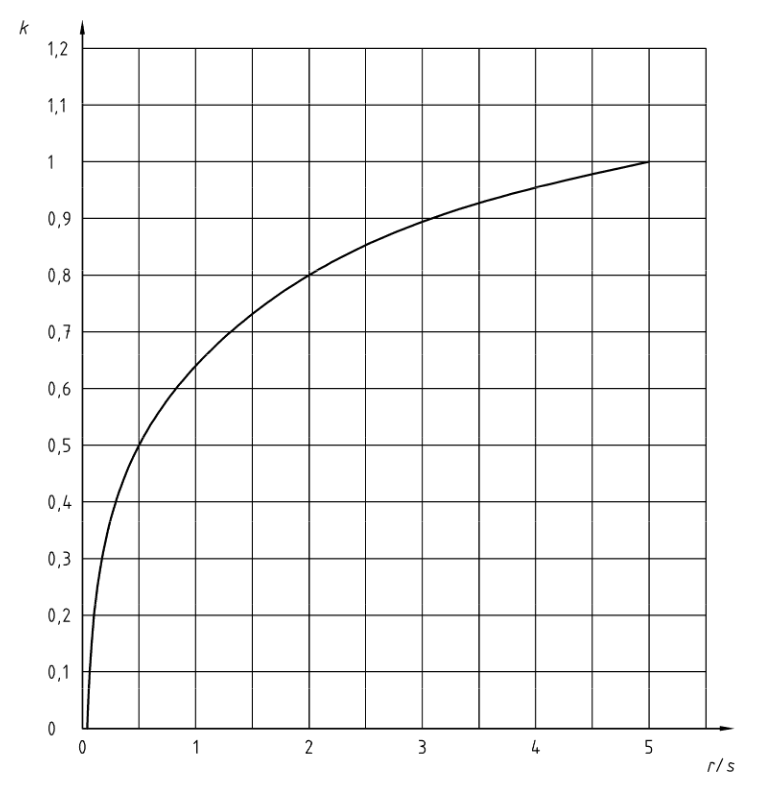
\includegraphics[width=0.5\linewidth]{k-factor}
% 	\caption[Graphical representation of the correction factor]{Graphical representation of the
% correction factor.}
% 	\label{fig:test1}
% \end{figure}

% The DIN 6935 used the formula for the stretched length, $length=a+b+v$ where \textit{a} and
% \textit{b} are the side
% lengths of the sheet and \textit{v} is a correction value for the deduction. \cite{din6935}
% The stretched length is measured different depending on the bending angle.

% \paragraph{Opening angle $\beta 0^\circ$ to $90^\circ$} 
% For opening angles between $0^\circ$and $90^\circ$ the side lengths \textit{a} and \textit{b}
% are dimensioned from
% the tangent of the bend to the edge.
% To calculate the compensation value \textit{v} (Equation~\ref{eq:v1}) is used
% \cite{din6935}.

% \begin{equation}\label{eq:v1}
%         v=\pi*(\frac{180^\circ-}{180^\circ})*(r+\frac{s}{2}*k)-2(r+s)
% \end{equation}

% \begin{figure}[H]
% 	\centering
% 	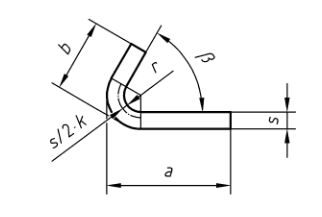
\includegraphics[width=0.5\linewidth]{bending-angle-90}
% 	\caption[Opening angles $\beta 0^\circ$ to $90^\circ$]{Opening angles $\beta 0^\circ$ to
% $90^\circ$ \cite{din6935}}
% 	\label{fig:v1-image}
% \end{figure}

% \paragraph{Bending angle $\beta90^\circ$ to $165^\circ$} (Equation~\ref{eq:v1})
% For opening angles between $90^\circ$ and $165^\circ$ the side lengths \textit{a} and
% \textit{b} are dimensioned
% from the apex to the edge.
% To calculate the compensation value \textit{v} (Equation~\ref{eq:v1}) is used. 
% \cite{din6935}

% \begin{equation}\label{eq:v2}
%     v=\pi*(\frac{180^\circ-}{180^\circ})*(r+\frac{s}{2}*k)-2(r+s)+\tan{\frac{180^\circ-\beta}{2}}
% \end{equation}

% \begin{figure}[!ht]
% 	\centering
% 	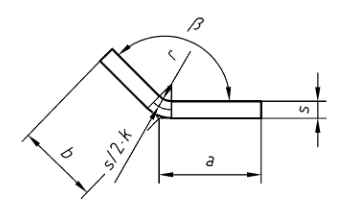
\includegraphics[width=0.5\linewidth]{bending-angle-165}
% 	\caption[Opening angles $\beta90^\circ$ to $165^\circ$]{Opening angles $\beta90^\circ$ to
% $165^\circ$
% \cite{din6935}}
% 	\label{fig:v2-image}
% \end{figure}

% For opening angles between $165^\circ$ and $180^\circ$ the compensation value \textit{v} is 0.
% The values for v
% would be negligibly small. \cite{din6935} The side lengths \textit{a} and \textit{b} where
% measured using the
% software \textit{ImageJ}.

% Edge cracking is not measured for now because the steel used has no high-strength and with
% machine in usage it was
% not possible to create edge cracking.

% \begin{figure}[!ht]
% 	\centering
% 	\includegraphics[width=0.5\linewidth]{example-image}
% 	\caption[Screenshot ImageJ]{Screenshot ImageJ}
% \end{figure}
% 	\label{fig:imagej-screenshot}